\documentclass[11pt,letterpaper]{article}
\pdfoutput=1
\usepackage{jheppub}
\usepackage[T1]{fontenc}
\usepackage[utf8]{inputenc}
\usepackage{amsthm,mathtools,booktabs,adjustbox,braket,enumitem,microtype}
\usepackage{bm}
\newcommand{\E}{\mathbb{E}}
\newcommand{\Prob}{\mathbb{P}}
\DeclareMathOperator{\Var}{Var}
\DeclareMathOperator{\Cov}{Cov}
\DeclareMathOperator{\tr}{tr}
\newcommand{\dd}{\mathrm{d}}
\theoremstyle{plain}
\newtheorem{theorem}{Theorem}[section]
\newtheorem{proposition}[theorem]{Proposition}
\newtheorem{lemma}[theorem]{Lemma}
\newtheorem{corollary}[theorem]{Corollary}
\theoremstyle{definition}
\newtheorem{definition}[theorem]{Definition}
\newtheorem{assumption}[theorem]{Assumption}
\theoremstyle{remark}
\newtheorem{remark}[theorem]{Remark}
\hypersetup{pdftitle={The Page Curve in Higher Dimensions: Phase Transitions, Critical Phenomena, and Finite-Size Broadening},
pdfauthor={Bernd Johannes Wuebben},
pdfsubject={Entanglement transitions and finite-size critical thermodynamics},
pdfkeywords={Page transition, charged AdS black holes, finite-size scaling, canonical ensemble}}
\preprint{\normalfont\small February 11, 2026 \textperiodcentered{} This version: October 10, 2026}
\title{The Page Curve in Higher Dimensions:\\
Phase Transitions, Critical Phenomena,\\
and Finite-Size Broadening}
\author{Bernd Johannes Wuebben}
\affiliation{New York, NY, USA}
\emailAdd{wuebben@gmail.com}
\abstract{Thermodynamic fluctuations round an entanglement transition on a scale set by the square root of a heat capacity away from criticality. At a charged AdS critical point this Gaussian approximation fails. We study its finite-size replacement in a canonical random-pure-state model whose density of states is given by the Reissner--Nordstr\"om--AdS entropy. In bulk dimension $d+1\geq4$, the critical entropy fluctuation is of order $S_c^{3/4}$ and has a quartic limiting distribution. We derive its coefficients, the full leading transition profile, and the thermal crossover in the window $|T-T_c|/T_c=O(S_c^{-3/4})$. An exact reduced action in four dimensions permits direct finite-size checks. Neutral AdS and BTZ examples provide the regular-phase comparison. A reservoir of finite heat capacity changes this distribution; the canonical critical limit requires reservoir heat capacity much larger than $S_c^{3/2}$. We distinguish this continuous critical crossover from a metastable spinodal and from first-order phase coexistence. We also separate thermodynamic entropy fluctuations from canonical modular-energy fluctuations and compute their distinct non-Gaussian corrections. The entanglement conclusions are exact asymptotic statements within the specified planar random-state model; applications to gravitational entropy transitions require the corresponding state and entropy-difference distribution.}
\keywords{Black holes, entanglement entropy, finite-size scaling, AdS thermodynamics}
\begin{document}
\hypersetup{pageanchor=false}
\notoc
\maketitle
\par\bigskip
{\small\noindent\textbf{Revision note (October 10, 2026).}
This version substantially revises the analysis of critical fluctuations and ensemble dependence. It derives the finite-size critical crossover, clarifies the random-state model underlying the entanglement calculation, and supersedes the broader universality claims of the earlier version.\par}
\clearpage
\pagenumbering{roman}
\hypersetup{pageanchor=true}
\newpage
\tableofcontents
\newpage
\pagenumbering{arabic}
\emergencystretch=2em

\section{Introduction}
\label{sec01:introduction}

Black-hole entropy and Hawking radiation connect equilibrium thermodynamics to a quantum-information question: how does the entropy of a subsystem change as information is redistributed between it and a black hole? The Bekenstein--Hawking entropy supplies the thermodynamic state count~\cite{bekenstein1973,hawking1975}, whereas Page's random-state calculation describes the entanglement of two systems with fixed Hilbert-space dimensions~\cite{page1993}. An evaporation model additionally prescribes how the available states and radiation change with time~\cite{page2013}. The transition region can already be studied as a function of subsystem size, before introducing this dynamical input. Its shape depends on the fluctuations present in the chosen state.

The leading approximation to an entanglement transition often selects the smaller of two entropy branches. The resulting corner is smoothed by fluctuations. For a random pure state with fixed subsystem dimensions, the correction at the Page transition is of order one~\cite{page1993}. In a thermodynamic state, fluctuations of the competing entropies can produce a parametrically larger correction. Murthy and Srednicki derived a square-root correction for chaotic energy eigenstates away from criticality~\cite{murthysrednicki2019}. Marolf, Wang and Wang formulated the corresponding diagonal approximation for holographic entropy transitions using fixed-area states~\cite{marolfwangwang2020}, and Dong and Wang obtained an enhanced correction by summing replica saddles in a chaotic holographic example~\cite{dongwang2020}. These results make the distribution of the entropy difference, including the constraints on that distribution, central to the transition.

Black-hole thermodynamics provides a setting in which the usual Gaussian approximation has a definite limit of validity. Spherical charged AdS black holes exhibit a line of small--large black-hole transitions ending at a continuous critical point~\cite{chamblin1999,kubiznakmann2012}. At the endpoint, the quadratic restoring term vanishes. Inserting the divergent saddle-point heat capacity into a Gaussian entropy profile does not define a finite-size transition. The next nonzero term in the thermodynamic action must be retained.

This paper determines the resulting entropy profile in a specified canonical model. Its black-hole sector has density of states proportional to $e^{S(E)}$, with $S(E)$ the Bekenstein--Hawking entropy of the chosen black-hole family. The charged-critical calculation uses the physical outer-horizon family of Reissner--Nordstr\"om--AdS solutions; the regular-phase examples use neutral AdS and nonrotating BTZ solutions. A $k$-dimensional reference system is entangled with this sector by a canonically weighted Gaussian random pure state. The control variable is $\log k$; no evaporation law is assumed. The planar reduced spectrum defines the entanglement entropy in this model. Its leading broad-distribution limit is the average of the smaller of $\log k$ and the canonical modular energy $K(E)=\beta E+\log Z$. This construction gives a precise meaning to the entropy transition and to the probability law over which it is averaged.

Our principal result is the finite-size replacement of the Gaussian profile at the charged critical point. Let $N=S_c$ be the critical black-hole entropy and take $N\to\infty$ at fixed critical geometry. In bulk dimension $d+1\geq4$, define
\begin{equation}
 a_d=\frac{(d-1)(2d-3)}{24},\qquad
 L_N=(d-1)a_d^{-1/4}N^{3/4}.
 \label{eq01:scale}
\end{equation}
The centered thermodynamic entropy and centered canonical modular energy, divided by $L_N$, have the same limiting law at criticality:
\begin{equation}
 p_0(X)=\frac{2}{\Gamma(1/4)}e^{-X^4}.
 \label{eq01:quartic}
\end{equation}
The entropy deficit relative to the minimum of the two mean branches is therefore of order $N^{3/4}$. Its ratio to the standard deviation at the crossing is $2^{-5/4}$, whereas the Gaussian ratio is $1/\sqrt{2\pi}$. The absolute width grows faster than in a regular phase, but its ratio to the black-hole entropy decreases as $N^{-1/4}$.

The same expansion determines a thermal scaling function. With $t=(T-T_c)/T_c$ and $h=L_Nt$ fixed, the limiting density is proportional to $e^{-X^4+hX}$. It gives a finite crossover through $t=0$ and matches the Gaussian width proportional to $N^{1/2}|t|^{-1/3}$ outside the critical window. In four bulk dimensions, the critical reduced action has the exact form
\begin{equation}
 \frac{I(r)-I(r_c)}{N}=\frac{(R-1)^4}{4R},\qquad R=\frac r{r_c},
 \label{eq01:exact_action}
\end{equation}
which makes the finite-size convergence directly calculable. Section~\ref{sec03:critical} derives these results and compares the limiting profiles with the full one-dimensional canonical integrals.

The preparation of the state matters even at leading order. At fixed total energy, exchange with a reservoir of heat capacity $C_R$ contributes a quadratic term to the critical distribution. The crossover occurs when $C_R$ is of order $N^{3/2}$; an ordinary extensive reservoir is too small to reproduce the canonical critical law. Away from criticality, the variance of the black-hole entropy is, to leading Gaussian order, the effective heat capacity $(C_B^{-1}+C_R^{-1})^{-1}$, while the difference between black-hole and reservoir entropies has four times that variance. Section~\ref{sec04:reservoir} derives both statements. They distinguish fixing the black-hole energy from fixing the total energy of two exchanging systems.

The regular-phase calculation provides a useful reference for these results. In a single stable phase, energy fluctuations have leading variance $T^2C$, so the entropy fluctuation has width $\sqrt C$. For large neutral AdS black holes, $C/S\to d-1$ as $r_+/\ell\to\infty$; the coefficient depends on dimension even though the square-root scaling is common. Section~\ref{sec10:regular} derives the Gaussian transition profile and its sensitivities, works through explicit examples, and compares them with the nonrotating BTZ thermodynamics~\cite{banados1992}. The BTZ equality $C=S$ fixes the leading fluctuation scale. It does not make thermodynamic entropy and canonical modular energy interchangeable at higher order. Appendix~\ref{app11:thermodynamics} supplies the thermodynamic derivations and distinguishes the large-radius limit from the semiclassical limit at fixed geometry.

Two other thermodynamic phenomena require separate treatments. The Schwarzschild--AdS minimum temperature is a spinodal of the black-hole branch, not the Hawking--Page coexistence temperature~\cite{hawkingpage1983}. Near the spinodal the Gaussian expansion fails before its extrapolated width becomes extensive. At first-order coexistence, by contrast, an equilibrium mixture can have an extensive width because the two phase means differ extensively. Section~\ref{sec05:phases} places these mechanisms alongside the charged critical crossover. Section~\ref{sec06:cumulants} gives the non-Gaussian expansion in a regular phase and explains why the cumulants of $S(E)$ cannot be substituted for those of $K(E)$ beyond their common leading variance.

The scope of the entanglement result is narrower than a general statement about evaporating AdS black holes. Quantum extremal surfaces and replica wormholes provide gravitational constructions of entropy transitions~\cite{engelhardtwall2015,penington2020,almheiri2020,pssy2022}. Applying the present thermodynamic distribution in such a construction requires an identification of the fluctuating difference of generalized entropies and of the allowed constraints. In particular, a critical mode shared by both branches may cancel from their difference. The model studied here specifies that difference and has a nonzero coupling to the critical mode. Section~\ref{sec02:model} states the model and the imported planar-spectrum result before any use of its entropy profile.

Charged AdS criticality, its quartic thermodynamic expansion, and enhanced entropy corrections each have substantial prior literature. Studies of charged AdS islands have examined the effect of thermodynamic phase transitions on Page curves~\cite{lin2024}; work on stochastic black-hole thermodynamics has examined critical relaxation and scaling~\cite{awal2026}. Our focus is the finite-entropy probability distribution at the endpoint, its induced entanglement profile in the specified model, and the reservoir scale required to retain it. We do not assign a new critical universality class to the charged black hole. The accompanying calculation of the planar correction uses the broad-distribution theorem of the companion paper~\cite{wuebben2026}, restated in Section~\ref{sec02:model}. That correction remains of order one and does not change the critical exponent.

Several distinctions organize the comparison with the existing literature. Hawking--Page thermodynamics and its gauge-theory interpretation concern the relative weights of different macroscopic phases~\cite{hawkingpage1983,witten1998}. The critical expansion considered here instead concerns fluctuations within a charged family at the endpoint of a coexistence line. In either setting, a state with a specified temperature need not have the same fluctuations as a state with a specified total energy. The stable finite-reservoir construction is related to the thermodynamic treatment of a black hole in a cavity~\cite{york1986}, but the entropy observable must still be identified before a capacity becomes a Page-transition width. These distinctions remain relevant even when the leading equilibrium geometry is the same.

There is also a distinction between fixing a geometric entropy and averaging over it. Fixed-area constructions clarify how semiclassical states with different area fluctuations can have different R\'enyi spectra~\cite{dong2019,akers2019}. The present planar model specifies both the canonical weights and the reduced spectrum, so that the averaging approximation can be compared with a defined entropy. For a gravitational application, the corresponding distribution over competing generalized entropies must be supplied by the state. Section~\ref{sec07:discussion} develops this interpretation, compares the fluctuation regimes, and identifies the additional dynamical input needed to convert an entropy width into a time interval.

The main contribution is thus the charged-critical finite-size crossover and its reservoir dependence. The regular thermodynamics, Gaussian identities, and dimensional examples provide the baseline needed to interpret it; the non-Gaussian expansion in Section~\ref{sec06:cumulants} explains how the thermodynamic and modular observables begin to differ away from criticality. The appendices collect the thermodynamic formulas, exact integrated identities, and stationary entropy-cost calculation so that these supporting results can be checked without consulting a companion manuscript.

\section{Entropy fluctuations and a canonical random-state model}
\label{sec02:model}

We first specify the relation between a probability distribution of thermodynamic fluctuations and an entanglement transition. Two distinct statements will be used. Averaging the smaller of two entropy branches gives a simple function of their difference. For the canonical random-state model defined below, a planar spectral calculation also determines the error of this averaging prescription. The thermodynamic calculations in the subsequent sections supply the probability distribution; they do not, by themselves, establish either prescription for an arbitrary gravitational state.

\subsection{The entropy difference and its probability distribution}

Let $S_1$ and $S_2$ be integrable random variables representing two competing entropy branches. The identity
\begin{equation}
 \E\min(S_1,S_2)
 =\frac{\E S_1+\E S_2}{2}-\frac12\E|S_1-S_2|
 \label{eq02:two_branches}
\end{equation}
shows that only the distribution of their difference enters the correction to the minimum of their means. In particular, the relevant variance is
\begin{equation}
 \sigma_{\mathrm{gap}}^2
 =\Var S_1+\Var S_2-2\Cov(S_1,S_2).
 \label{eq02:gap_variance}
\end{equation}
A fluctuation common to both branches cancels. A heat capacity can therefore determine a transition width only after the coupling of the fluctuating thermodynamic variable to the entropy difference has been specified.

For a fixed centered fluctuation $\xi$, define the averaged minimum and its deficit by
\begin{align}
 M(\Delta)&=\E\min(\Delta,\xi),
 \label{eq02:averaged_minimum}\\
 B(\Delta)&=\min(\Delta,0)-M(\Delta)
 =\frac12\bigl(\E|\Delta-\xi|-|\Delta|\bigr).
 \label{eq02:deficit}
\end{align}
Here $\Delta$ translates the mean difference while the fluctuation law is held fixed. Convexity gives $B\geq0$. If $F$ is the cumulative distribution function of $\xi$, then $B'=F$ for $\Delta<0$ and $B'=F-1$ for $\Delta>0$, at points of differentiability. Consequently the deficit is largest at the crossing of the means, even for an asymmetric distribution, and
\begin{equation}
 B(0)=\frac12\E|\xi|\leq\frac{\sigma}{2},
 \qquad \sigma^2=\E\xi^2.
 \label{eq02:central_deficit}
\end{equation}
The curvature has a particularly direct interpretation. If $\xi$ has density $p_\xi$, then
\begin{equation}
 -M''(\Delta)=p_\xi(\Delta).
 \label{eq02:curvature}
\end{equation}
These identities are exact for the averaged minimum. They are not identities for every quantum entropy. Appendix~\ref{app08:identities} gives their integrated forms and the modification produced by the fixed-area Page correction.

For a Gaussian fluctuation, writing $z=\Delta/\sigma$, one obtains
\begin{equation}
 M_{\mathrm G}(\Delta)=\Delta\Phi(-z)-\sigma\phi(z),
 \qquad B_{\mathrm G}(0)=\frac{\sigma}{\sqrt{2\pi}},
 \label{eq02:gaussian}
\end{equation}
where $\phi$ and $\Phi$ are the standard normal density and distribution function. The same averaging of competing extensive entropies underlies the enhanced corrections found for chaotic energy eigenstates and for holographic entanglement transitions~\cite{murthysrednicki2019,marolfwangwang2020,dongwang2020}. Our main concern is the replacement of this Gaussian law near a thermodynamic critical point.

\subsection{Canonical probabilities and random pure states}

Let the black-hole system have energy levels $E_j$, with finite canonical partition function and mean energy,
\begin{equation}
 Z(\beta)=\sum_j e^{-\beta E_j},\qquad
 x_j=\frac{e^{-\beta E_j}}{Z(\beta)},\qquad
 K_j=-\log x_j=\beta E_j+\log Z.
 \label{eq02:canonical_levels}
\end{equation}
The random variable $K$ is sampled with probabilities $x_j$. It is the modular energy of a canonical density-matrix eigenstate, and its mean is the canonical von Neumann entropy $S_{\mathrm{can}}=\E K$. All logarithms are natural and entropies are measured in nats.

Take a reference system of dimension $k$, set $s=\log k$, and consider the pure-state ensemble
\begin{equation}
 |\Psi\rangle=
 \frac{1}{\sqrt{\mathcal N}}
 \sum_{i=1}^{k}\sum_j \sqrt{x_j}\,g_{ij}
 |i\rangle_R|j\rangle_B,
 \qquad
 \mathcal N=\sum_{i,j}x_j|g_{ij}|^2,
 \label{eq02:random_state}
\end{equation}
where the $g_{ij}$ are independent complex Gaussian variables of unit variance. The reduced reference state is a normalized weighted Wishart matrix. The reference dimension is an independent control parameter; the model does not impose energy conservation between the reference and the black hole.

We use the planar spectral description of this ensemble, familiar from canonical random-state and replica calculations~\cite{pssy2022,wuebben2026}. More precisely, the planar model is defined by the probability law $\nu$ of rescaled reference eigenvalues $u=k\lambda$, whose $R$-transform is
\begin{equation}
 R_\nu(w)=\E_P\frac{1}{1-aw},\qquad
 a=kx_j=e^{s-K_j},\qquad P\{a=kx_j\}=x_j.
 \label{eq02:r_transform}
\end{equation}
Equivalently, its free cumulants are $\kappa_n^{\mathrm{free}}=\E_P a^{n-1}$ whenever these moments exist. In resolvent notation, $g_\nu(z)=\int(z-u)^{-1}\nu(\dd u)$ satisfies $z=1/g_\nu(z)+R_\nu(g_\nu(z))$ on the branch with $g_\nu(z)\sim1/z$ at infinity. This normalization gives $\int u\,\nu(\dd u)=1$. The planar entropy is
\begin{equation}
 S_{\mathrm{planar}}=s-\int_0^\infty u\log u\,\nu(\dd u).
 \label{eq02:planar_entropy}
\end{equation}
Equation~\eqref{eq02:r_transform} specifies the spectrum used here; no simultaneous theorem concerning the finite matrix size and the gravitational semiclassical limit is assumed.

For $L$ equiprobable black-hole levels, $P$ is a single atom at $a=k/L$. The Marchenko--Pastur entropy then gives the planar limit of Page's result~\cite{page1993},
\begin{equation}
 S_{\mathrm{fixed}}(s,\log L)
 =\min(s,\log L)-\frac12e^{-|s-\log L|}.
 \label{eq02:fixed_page}
\end{equation}
This motivates the level-resolved diagonal approximation
\begin{equation}
 S_{\mathrm{diag}}
 =\E\left[\min(s,K)-\frac12e^{-|s-K|}\right].
 \label{eq02:diagonal}
\end{equation}
It is an explicitly defined approximation to~\eqref{eq02:planar_entropy}, not the entropy of an orthogonal decomposition into energy sectors. With $\xi=K-S_{\mathrm{can}}$ and $\Delta=s-S_{\mathrm{can}}$, its leading term is $S_{\mathrm{can}}+M(\Delta)$.

The distinction between the exact planar spectrum and the diagonal Page approximation remains bounded for broad distributions. We use the following result of the companion paper~\cite{wuebben2026}.

\begin{proposition}[Broad canonical distributions]
\label{prop02:spreading}
For a family of laws $P_N$ in~\eqref{eq02:r_transform}, suppose $\E_{P_N}a<\infty$ and set $\delta=-\log a=K-s$. Assume that, for every fixed $A>0$,
\begin{equation}
 \Prob_N(|\delta|\leq A)\longrightarrow0,
 \qquad
 w_{>,N}=\Prob_N(\delta>0)\longrightarrow w_>\in(0,1).
 \label{eq02:spreading}
\end{equation}
Then
\begin{equation}
 S_{\mathrm{planar}}-S_{\mathrm{diag}}
 \longrightarrow -w_>\log w_>.
 \label{eq02:planar_gap}
\end{equation}
\end{proposition}

For completeness, Appendix~\ref{app08:identities} records the resolvent integral from which this limit follows. The result does not require a Gaussian distribution. In particular, if $(K-S_{\mathrm{can}})/L_N$ converges to a continuous symmetric law, $L_N\to\infty$, and the transition is centered at $s=S_{\mathrm{can}}$, the limit is $\tfrac12\log2$. The canonical weight in levels with $x_j\ll1/k$ is spread over the entire reference space. It produces an approximately uniform contribution of total weight $w_>$ to the reference spectrum, whose entropy includes $-w_>\log w_>$. Averaging the fixed-dimension Page formula omits this term.

Under~\eqref{eq02:spreading}, the exponential term in~\eqref{eq02:diagonal} tends to zero by bounded convergence in probability. Thus, whenever the absolute first moments also converge after division by $L_N$, the averaged minimum determines the leading $O(L_N)$ entropy deficit, and~\eqref{eq02:planar_gap} determines its additive planar correction relative to the \emph{full} diagonal approximation. Subleading thermodynamic contributions to $M$ can be larger than one nat; the limit does not remove them.

\subsection{The thermodynamic density of states and gravitational scope}

For the thermodynamic calculations, the level count is modeled by
\begin{equation}
 \dd n(E)=e^{S(E)}\frac{\dd E}{E_0},\qquad
 Z=\int e^{S(E)-\beta E}\frac{\dd E}{E_0},\qquad
 p_\beta(E)=\frac{e^{S(E)-\beta E}}{E_0Z},
 \label{eq02:density_of_states}
\end{equation}
on a specified physical energy domain. The constant $E_0$ fixes the energy unit in the density of states. In the black-hole examples, $S(E)$ is the Bekenstein--Hawking entropy evaluated along the chosen family of geometries. This is a defined density-of-states model; a gravitational determinant or a competing matter phase is not supplied by~\eqref{eq02:density_of_states}.

The thermodynamic entropy $S(E)$ and the canonical modular energy $K(E)$ are different functions. If
\begin{equation}
 I(E)=\beta E-S(E),
 \qquad K(E)-S(E)=I(E)+\log Z,
 \label{eq02:action_dictionary}
\end{equation}
then their centered difference obeys the exact relation
\begin{equation}
 \bigl(K-\E K\bigr)-\bigl(S-\E S\bigr)=I-\E I.
 \label{eq02:centered_dictionary}
\end{equation}
At a well-controlled quadratic or quartic saddle, action fluctuations remain of order one. Both centered variables therefore have the same leading broad distribution, although their higher cumulants and subleading corrections need not agree. Section~\ref{sec06:cumulants} makes this distinction explicit away from criticality.

An application to a generalized-entropy transition requires a state and ensemble for which averaging two competing branches is valid at the order considered~\cite{engelhardtwall2015,marolfwangwang2020,dongwang2020}. It also requires the response of their \emph{difference} to the fluctuating mode. For example, if that difference is $g(E)$ and $g'(E_c)\neq0$, a leading critical law for energy fluctuations is transferred to $g(E)$ by linearization. If the linear response vanishes, the width and limiting shape change. The canonical model~\eqref{eq02:random_state} supplies a definite nonzero response through $K'(E)=\beta$.

Energy-recording radiation gives a different construction: its reduced state can be an orthogonal sum over energy sectors. Section~\ref{sec04:reservoir} treats the resulting sector entropy and the constraints on energy exchange. The planar correction~\eqref{eq02:planar_gap} pertains to the common reference space in~\eqref{eq02:random_state}.

\section{Gaussian broadening in a stable black-hole phase}
\label{sec10:regular}

Before treating the charged critical point, we develop the noncritical limit of the model in Section~\ref{sec02:model}. This limit fixes the normalization of the entropy width and provides explicit comparisons across dimensions. Its Gaussian profile is the familiar enhanced correction to a transition between competing entropies~\cite{murthysrednicki2019,marolfwangwang2020,dongwang2020}. The calculation also identifies the assumptions that fail at a degenerate saddle or when a second phase has appreciable probability.

\subsection{The quadratic saddle and the entropy variable}

Let $E_*$ be a nondegenerate minimum of $I(E)=\beta E-S(E)$, and write $S_*=S(E_*)$. At fixed external charges and AdS length, the first law gives
\begin{equation}
 S'(E_*)=\frac1T,\qquad
 S''(E_*)=-\frac{1}{T^2C},\qquad
 C=\frac{\dd E_*}{\dd T}=T\frac{\dd S_*}{\dd T}>0.
 \label{eq10:quadratic_capacity}
\end{equation}
Here $C$ is the heat capacity of the classical saddle. We take a regular large-entropy limit with $C$ proportional to $S_*$, with the saddle separated from boundaries and competing phases. More precisely, the expansion of the action and its derivatives is assumed uniform on the fluctuation scale, with integrable tails sufficient for convergence of the moments used below. These conditions hold for the single dominant neutral black-hole saddle at fixed $r_+/\ell>1$ as $G\to0$ in the density model~\eqref{eq02:density_of_states}.

Writing $y=(E-E_*)/(T\sqrt C)$ gives
\begin{equation}
 I(E)-I(E_*)=\frac{y^2}{2}
 +O(S_*^{-1/2})\qquad (y\ \hbox{in a bounded interval}).
 \label{eq10:quadratic_action}
\end{equation}
The energy law therefore approaches a standard Gaussian in $y$. The linearized entropy fluctuation is $\delta S=(E-E_*)/T$, so its variance is $C$ at leading order. The canonical modular energy has the same linear response, $\delta K=\beta\delta E$. In particular,
\begin{equation}
 \frac{S-\E S}{\sqrt C}\ \Longrightarrow\ {\cal N}(0,1),
 \qquad
 \frac{K-S_{\mathrm{can}}}{\sqrt C}\ \Longrightarrow\ {\cal N}(0,1).
 \label{eq10:regular_limit}
\end{equation}
The equality is asymptotic. In the exact canonical model, differentiating $Z$ gives
\begin{equation}
 \Var K=\beta^2\Var E=C_{\mathrm{can}},\qquad
 C_{\mathrm{can}}=\frac{\dd\E E}{\dd T},
 \label{eq10:exact_capacity}
\end{equation}
whereas $\Var S=C+O(1)$ and $C_{\mathrm{can}}=C+O(1)$ under a regular saddle expansion. There is no exact identity equating $\Var S(E)$ to either heat capacity. Section~\ref{sec06:cumulants} develops the corresponding difference between their higher cumulants.

The mean about which the transition is centered also requires care. With the particular measure $\dd E/E_0$ specified in~\eqref{eq02:density_of_states}, Laplace's method yields
\begin{equation}
 \log Z=S_*-\beta E_*
 +\log\!\left(\frac{T\sqrt{2\pi C}}{E_0}\right)+O(S_*^{-1}).
 \label{eq10:partition_saddle}
\end{equation}
If the expansion can be differentiated uniformly in a neighborhood of $T$, the canonical mean is
\begin{equation}
 S_{\mathrm{can}}
 =S_*+\log\!\left(\frac{T\sqrt{2\pi C}}{E_0}\right)
 +1+\frac{TC'}{2C}+O(S_*^{-1}).
 \label{eq10:canonical_center}
\end{equation}
Indeed, $S_{\mathrm{can}}=(1+T\partial_T)\log Z$, and the derivative of the logarithmic prefactor is $1+TC'/(2C)$. The shift is smaller than the $\sqrt{S_*}$ width but matters at logarithmic and constant accuracy. For example, in four bulk dimensions with $r_+/\ell=2$, $S_*=100$, and $E_0\ell=1$, direct integration over the neutral black-hole family gives $S_{\mathrm{can}}=104.975702$ and $\Var K=238.438623$, compared with the saddle value $C=236.363636$. A different density-of-states prefactor changes these subleading numbers; the leading Gaussian width survives when that prefactor is locally constant on the scaled fluctuation interval and the tails remain controlled.

\subsection{The transition profile and its derivatives}

Set $\mu=S_{\mathrm{can}}$, $\sigma=\sqrt C$ at leading order, and $z=(s-\mu)/\sigma$. Substitution of the Gaussian limit into the averaged minimum gives
\begin{equation}
 {\cal S}_{\mathrm G}(s;\mu,\sigma)
 =s\Phi(-z)+\mu\Phi(z)-\sigma\phi(z).
 \label{eq10:full_gaussian_profile}
\end{equation}
For bounded $z$, the actual averaged minimum differs from~\eqref{eq10:full_gaussian_profile} by $o(\sqrt C)$ when the first absolute moments converge in~\eqref{eq10:regular_limit}. Thus~\eqref{eq10:full_gaussian_profile} is the full leading crossover, rather than just the deficit at its center. It approaches the reference entropy $s$ on one side and the canonical entropy $\mu$ on the other. The positive deficit from their smaller value is
\begin{equation}
 B_{\mathrm G}(\Delta)
 =\sigma\phi\!\left(\frac{|\Delta|}{\sigma}\right)
 -|\Delta|\Phi\!\left(-\frac{|\Delta|}{\sigma}\right),
 \qquad \Delta=s-\mu.
 \label{eq10:gaussian_deficit}
\end{equation}
In particular, $B_{\mathrm G}(0)=\sqrt{C/(2\pi)}$. Under the spreading hypotheses of Proposition~\ref{prop02:spreading}, the planar entropy and the diagonal entropy have the same leading $\sqrt C$ profile. Their bounded difference is treated separately in~\eqref{eq02:planar_gap}; it does not change this leading scale.

The complete Gaussian average of the diagonal Page kernel can also be evaluated in closed form; Appendix~\ref{app08:gaussian} gives the exponential term in~\eqref{eq08:gaussian_kernel}. Its central contribution to the entropy is of order $1/\sigma$. That term and the order-one planar correction refer to different differences of entropies, and neither is included in the leading expression~\eqref{eq10:full_gaussian_profile}.

The partial derivatives give useful ways to describe the crossover. Holding the other displayed parameters fixed,
\begin{equation}
 \frac{\partial{\cal S}_{\mathrm G}}{\partial s}=\Phi(-z),
 \qquad
 \frac{\partial{\cal S}_{\mathrm G}}{\partial\mu}=\Phi(z),
 \qquad
 \frac{\partial{\cal S}_{\mathrm G}}{\partial\sigma}=-\phi(z),
 \qquad
 \frac{\partial^2{\cal S}_{\mathrm G}}{\partial s^2}
 =-\frac{\phi(z)}{\sigma}.
 \label{eq10:gaussian_sensitivities}
\end{equation}
Consequently increasing $\sigma$ at fixed means increases the deficit, and the curvature resolves the Gaussian fluctuation density. The slope falls from $0.9$ to $0.1$ across an entropy interval $2\Phi^{-1}(0.9)\sigma=2.563103\sigma$. This is one operational definition of a crossover width; the standard deviation $\sigma$ is the convention used elsewhere in the paper.

At $s=\mu$, the slope in~\eqref{eq10:gaussian_sensitivities} is one half because the fluctuation law is symmetric. This is a derivative with respect to the reference entropy while its canonical distribution is fixed. Varying a physical temperature changes both $\mu$ and $\sigma$; evolving a coupled system can change the entire distribution. Neither the half-slope nor $\sigma$ alone specifies an entropy-production rate or a duration in time. The same distinction applies to the non-Gaussian profiles below.

\subsection{Neutral AdS black holes in different dimensions}

For a Schwarzschild--AdS black hole in bulk dimension $d+1\geq4$, set $y_+=r_+/\ell$. The thermodynamic formulas derived in Appendix~\ref{app11:thermodynamics} give
\begin{equation}
 S_* =\frac{\Omega_{d-1}r_+^{d-1}}{4G},\qquad
 T=\frac{d-2+d y_+^2}{4\pi r_+},\qquad
 \frac{C}{S_*}=(d-1)\frac{d y_+^2+d-2}{d y_+^2-d+2}.
 \label{eq10:neutral_width}
\end{equation}
Here $\Omega_{d-1}$ is the area of the unit $(d-1)$-sphere, and the derivative defining $C$ holds $\ell$ fixed. The large-black-hole branch has $y_+>\sqrt{(d-2)/d}$. We first restrict to fixed $y_+>1$, where the black-hole free energy is lower than thermal AdS and the usual Hawking--Page competition does not affect the leading single-phase distribution~\cite{hawkingpage1983,witten1998}. The metastable interval below $y_+=1$ and the coexistence region require the distinctions made in Section~\ref{sec05:phases}.

There are two separate approximations in the frequently used expression $\sigma\simeq\sqrt{(d-1)S_*}$. The large-radius expansion is
\begin{equation}
 \frac{C}{S_*}
 =(d-1)\left[1+\frac{2(d-2)}{d}\frac{\ell^2}{r_+^2}
 +O\!\left(\frac{\ell^4}{r_+^4}\right)\right].
 \label{eq10:large_radius}
\end{equation}
This is an expansion in $\ell/r_+$, independent of the expansion in quantum fluctuations. At fixed $r_+/\ell>1$, taking $G\to0$ makes $S_*$ and $C$ large and makes the Gaussian approximation accurate, but it leaves the geometric correction in~\eqref{eq10:large_radius} unchanged. In contrast, increasing $r_+$ at fixed $G$ and $\ell$ suppresses that correction as $S_*^{-2/(d-1)}$, with a coefficient that depends on the fixed parameters. Large entropy alone does not justify replacing $C/S_*$ by $d-1$.

\begin{table}[t]
 \centering
 \caption{Regular Gaussian widths at $r_+/\ell=2$, evaluated from~\eqref{eq10:neutral_width}. All entries refer to the leading large-$S_*$ distribution within one black-hole phase. The final column is the distinct limit $r_+/\ell\to\infty$. Widths are compared at the same entropy $S_*$, not at the same mass or Newton constant across different dimensions.}
 \label{tab10:dimensions}
 \begin{adjustbox}{max width=\textwidth}
 \begin{tabular}{@{}ccccc@{}}
 \toprule
 Bulk dimension & $C/S_*$ & $\sigma/\sqrt{S_*}$ & $B_{\mathrm G}(0)/\sqrt{S_*}$ & $\lim_{r_+/\ell\to\infty}\sigma/\sqrt{S_*}$\\
 \midrule
 $4$ & $26/11$ & $1.537412$ & $0.613339$ & $\sqrt2$\\
 $5$ & $27/7$ & $1.963961$ & $0.783507$ & $\sqrt3$\\
 $6$ & $92/17$ & $2.326320$ & $0.928067$ & $2$\\
 $7$ & $7$ & $2.645751$ & $1.055502$ & $\sqrt5$\\
 \bottomrule
 \end{tabular}
 \end{adjustbox}
\end{table}

Table~\ref{tab10:dimensions} gives examples away from both limits of stability and phase competition. At fixed $S_*$ and $r_+/\ell$, the Gaussian width increases with the bulk dimension. In the large-radius limit this becomes the coefficient $\sqrt{d-1}$, reflecting the equation of state $S_*\propto T^{d-1}$. The deficit grows in absolute entropy units but decreases relative to the leading entropy:
\begin{equation}
 \frac{B_{\mathrm G}(0)}{S_*}
 =\sqrt{\frac{C/S_*}{2\pi S_*}}
 \longrightarrow0.
 \label{eq10:relative_width}
\end{equation}
Figure~\ref{fig10:regular} displays both the geometric dependence of the width and the resulting profile. These regular transitions provide the reference for the $S_c^{3/4}$ critical width in Section~\ref{sec03:critical}, whose relative size decreases more slowly.

\begin{figure}[t]
 \centering
 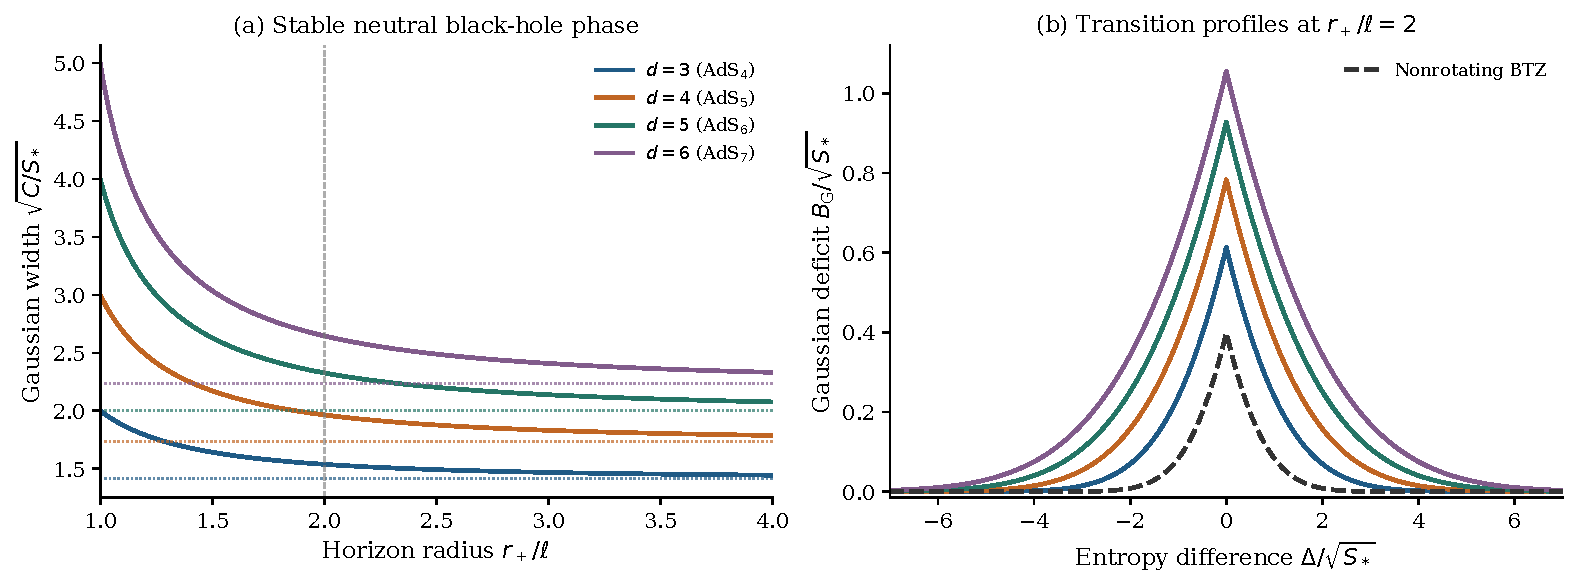
\includegraphics[width=\textwidth]{figures/output/jhep2_regular.pdf}
 \caption{Gaussian broadening within a stable black-hole phase. (a)~The leading entropy width divided by $\sqrt{S_*}$ for four bulk dimensions $d+1=4,5,6,7$. Dotted horizontal lines give the large-radius limits $\sqrt{d-1}$, and the vertical line marks $r_+/\ell=2$. Only $r_+/\ell>1$ is plotted. (b)~The averaged-minimum deficits at this radius, with the same colors as in (a), compared with the nonrotating BTZ result $C=S_*$. Both axes are scaled by $\sqrt{S_*}$, so the curves show the leading large-entropy profiles rather than finite-size quadrature. They evaluate~\eqref{eq10:gaussian_deficit} and~\eqref{eq10:neutral_width}; no gravitational replica calculation is represented.}
 \label{fig10:regular}
\end{figure}

\subsection{The nonrotating BTZ example}

The neutral, nonrotating BTZ black hole provides a useful lower-dimensional check~\cite{banados1992}. We hold angular momentum fixed at $J=0$ and use the mass convention in which the zero-radius BTZ solution has $E=0$:
\begin{equation}
 E=\frac{r_+^2}{8G_3\ell^2},\qquad
 S_* =\frac{\pi r_+}{2G_3},\qquad
 T=\frac{r_+}{2\pi\ell^2},\qquad
 C=S_* =\frac{\pi^2\ell^2}{G_3}T.
 \label{eq10:btz_thermodynamics}
\end{equation}
The relation $C=S_*$ is exact for these classical thermodynamic functions. Global AdS$_3$ has energy $-1/(8G_3)$ in the same convention. It is a separate saddle, and it competes with BTZ at $r_+=\ell$; the positive BTZ heat capacity at all radii does not eliminate this first-order competition. The energy reference and free energies are detailed in Appendix~\ref{app11:thermodynamics}.

The density model permits a more precise check than the leading identity $\sigma^2\simeq S_*$. Write its thermodynamic entropy as $S(E)=A\sqrt E$, where $A=\pi\ell\sqrt{2/G_3}$. Since $S_*=A^2T/2$, changing the integration variable from energy to entropy gives the exact probability law within the BTZ family,
\begin{equation}
 p_S(S)\propto S\exp\!\left[-\frac{(S-S_*)^2}{2S_*}\right],
 \qquad S>0.
 \label{eq10:btz_entropy_law}
\end{equation}
The factor $S$ is the Jacobian $\dd E=2S\,\dd S/A^2$. Thus the exponent is quadratic but the distribution is not exactly Gaussian. Its partition function, including the lower endpoint, is
\begin{equation}
 Z_{\mathrm{BTZ}}=\frac{T}{E_0}
 \left[1+\sqrt{2\pi S_*}\,e^{S_*/2}\Phi(\sqrt{S_*})\right].
 \label{eq10:btz_exact_partition}
\end{equation}
Keeping a fixed number of moments and taking $S_*\to\infty$ yields
\begin{equation}
 \E S=S_*+1+o(1),\qquad
 \Var S=S_*-1+o(1),\qquad
 \Var K=C_{\mathrm{can}}=S_*+\frac32+o(1).
 \label{eq10:btz_finite_terms}
\end{equation}
The remainders in~\eqref{eq10:btz_finite_terms} are exponentially small. To see the first two constants directly, set $S=S_*+\sqrt{S_*}\,y$ in~\eqref{eq10:btz_entropy_law}. Apart from the exponentially distant endpoint, its Gaussian weight is multiplied by $1+y/\sqrt{S_*}$, which shifts the mean by one and the variance by minus one. For the third result,~\eqref{eq10:btz_exact_partition} gives $\log Z_{\mathrm{BTZ}}=S_*/2+(3/2)\log T+\text{constant}+o(1)$ at fixed $G_3,\ell,E_0$; two temperature derivatives give $C_{\mathrm{can}}=S_*+3/2+o(1)$.

Likewise, because $S_*\propto T$, the leading extensive cumulants of the thermodynamic variable $S(E)$ vanish beyond second order, as follows from~\eqref{eq06:entropy_cumulants}. The modular energy has instead $\kappa_3[K]=3S_*+O(1)$ and $\kappa_4[K]=12S_*+O(1)$. These facts are compatible with the same Gaussian limit after division by $\sqrt{S_*}$. The finite constants in~\eqref{eq10:btz_finite_terms} belong to the specified measure $e^{S(E)}\dd E/E_0$; they are not asserted to be one-loop corrections to a complete BTZ or conformal-field-theory partition function. Summing over angular momentum at zero angular potential, rather than fixing $J=0$, also changes the fluctuation problem and its prefactors.

The leading density has the standard conformal-field-theory interpretation. With equal left and right Brown--Henneaux central charges $c=3\ell/(2G_3)$~\cite{brown1986}, define cylinder energies $n_L=h-c/24$ and $n_R=\bar h-c/24$ in terms of plane conformal weights. The dictionary and Cardy entropy are
\begin{equation}
 n_L+n_R=\ell E,\qquad n_L-n_R=J,\qquad
 S_{\mathrm{Cardy}}=2\pi\sqrt{\frac{c n_L}{6}}
                  +2\pi\sqrt{\frac{c n_R}{6}}.
 \label{eq10:cardy_dictionary}
\end{equation}
At $J=0$, substitution gives $S_{\mathrm{Cardy}}=A\sqrt E$, reproducing the leading BTZ entropy~\cite{cardy1986,strominger1998}. The shifts ensure that the plane vacuum $h=\bar h=0$ corresponds to global AdS$_3$, with $E=-c/(12\ell)=-1/(8G_3)$. Cardy's high-energy asymptotics applies under the usual unitary, modular-invariant conformal-field-theory assumptions, in a regime where the vacuum controls the modularly transformed partition function. A sufficient high-energy limit takes both $n_L/c$ and $n_R/c$ large; extending the formula to lower energies at large $c$ requires additional information about the spectrum. Accordingly, taking $G_3\to0$ at a fixed $r_+/\ell$ does not by itself establish the unrestricted Cardy approximation. This comparison verifies the leading thermodynamic input and its Gaussian scale. It neither fixes the subleading density prefactor nor identifies the entanglement state with a particular two-dimensional gravity model.

\section{The charged AdS critical point}
\label{sec03:critical}

The canonical critical point of a charged AdS black hole provides a
setting in which the entropy fluctuations are parametrically larger
than those of a nondegenerate saddle.  The relevant canonical action
has a quartic minimum.  The existence of this critical point and its
mean-field thermodynamics are established results
\cite{chamblin1999,kubiznakmann2012}; quartic free-energy expansions also
enter studies of its relaxation dynamics \cite{awal2026}.  Here we use
the equilibrium probability distribution at finite entropy to obtain
the complete leading rounding profile in the model of
section~\ref{sec02:model}.

\subsection{Thermodynamic model and critical geometry}

For a spherical Reissner--Nordstr\"om--AdS black hole in $d+1$
dimensions, $d\geq3$, choose the metric charge parameter $q$ so that
the horizon thermodynamics is
\begin{align}
 M(r)&=\frac{(d-1)\Omega_{d-1}}{16\pi G}
 \left(r^{d-2}+\frac{r^d}{\ell^2}
                  +\frac{q^2}{r^{d-2}}\right),
 \label{eq03:mass_entropy}\\
 S(r)&=\frac{\Omega_{d-1}r^{d-1}}{4G},
 \nonumber\\
 T_H(r)&=\frac{1}{4\pi r}
 \left(d-2+\frac{d r^2}{\ell^2}
              -\frac{(d-2)q^2}{r^{2d-4}}\right).
 \label{eq03:temperature}
\end{align}
Here $\Omega_{d-1}$ is the area of the unit $(d-1)$-sphere.  The AdS
length and charge are fixed, and $\dd M=T_H\dd S$.  We retain only the
outer-horizon branch $r\geq r_{\mathrm{ext}}$, where $T_H\geq0$ and
$M$ increases with $r$.  The canonical model is the density of states
\begin{equation}
 \rho(E)\,\dd E=e^{S(E)}\frac{\dd E}{E_0},\qquad
 Z_N(\beta)=\int_{M(r_{\mathrm{ext}})}^\infty
       e^{S(E)-\beta E}\frac{\dd E}{E_0},
 \label{eq03:dos}
\end{equation}
with a fixed reference energy $E_0$.  Thus the probability measure on
horizon radii contains the Jacobian $M'(r)\dd r$, rather than a flat
measure in $r$.  Equation~\eqref{eq03:dos} specifies a thermodynamic
model; it does not assert that the Bekenstein--Hawking entropy is the
complete quantum density of states.

The inflection conditions $T_H'(r_c)=T_H''(r_c)=0$ give
\begin{equation}
 r_c^2=\frac{(d-2)^2\ell^2}{d(d-1)},\qquad
 q_c^2=\frac{r_c^{2d-4}}{(2d-3)(d-1)},\qquad
 T_c=\frac{(d-2)^2}{\pi(2d-3)r_c}.
 \label{eq03:critical_geometry}
\end{equation}
We set $q=q_c$ and take $G\to0$ at fixed critical geometry, so that
\begin{equation}
 N=S(r_c)\longrightarrow\infty,\qquad
 R=\frac{r}{r_c},\qquad x=R-1.
 \label{eq03:size}
\end{equation}
The size parameter $N$ is the critical black-hole entropy, not a
gauge-group rank.

It is useful to verify that the critical saddle controls the whole
RN integral, rather than only a local expansion.  Put $n=d-2$.  At
the critical charge,
\begin{equation}
 \frac{T_H(R)}{T_c}
 =\frac{2n+1}{4n}
 \left(\frac{1}{R}+\frac{nR}{n+1}
       -\frac{R^{-2n-1}}{(2n+1)(n+1)}\right).
 \label{eq03:reduced_temperature}
\end{equation}
Its derivative has the sign of
\begin{equation}
 P(y)=n y^{n+1}-(n+1)y^n+1,\qquad y=R^2.
 \label{eq03:monotonic_polynomial}
\end{equation}
Since $P'(y)=n(n+1)y^{n-1}(y-1)$ and $P(1)=0$, one has
$P(y)>0$ for $y>0$, $y\neq1$.  Consequently $T_H(R)$ is strictly
increasing, with a stationary inflection at $R=1$.  For
$I_c(R)=\beta_c M(R)-S(R)$, the first law gives
\begin{equation}
 \frac{\dd I_c}{\dd R}
   =N(d-1)R^{d-2}\left(\frac{T_H(R)}{T_c}-1\right).
 \label{eq03:action_derivative}
\end{equation}
It follows that $I_c$ has a unique global minimum at $R=1$ on the
outer-horizon branch.  This conclusion concerns the RN family in
\eqref{eq03:dos}; it does not exclude competing matter phases or
instabilities outside that family.

\subsection{Quartic fluctuations and the rounding profile}

The first two derivatives of \eqref{eq03:reduced_temperature} vanish
at $R=1$, whereas its third derivative equals $2d-3$.  Integration
of \eqref{eq03:action_derivative} therefore yields
\begin{equation}
 I_c(R)-I_c(1)
 =N\left[a_d x^4+O(x^5)\right],\qquad
 a_d=\frac{(d-1)(2d-3)}{24}.
 \label{eq03:quartic_action}
\end{equation}
Define the dimensionless fluctuation and entropy scale
\begin{equation}
 X_N=(a_dN)^{1/4}(R-1),\qquad
 L_N=(d-1)a_d^{-1/4}N^{3/4}.
 \label{eq03:scales}
\end{equation}

\begin{proposition}[Critical entropy fluctuations]
\label{prop03:quartic}
In the canonical model \eqref{eq03:dos} at $\beta=\beta_c$,
$X_N$ converges in distribution and in every polynomial moment to
the density
\begin{equation}
 p_0(X)=\frac{2}{\Gamma(1/4)}e^{-X^4},
 \qquad -\infty<X<\infty.
 \label{eq03:quartic_density}
\end{equation}
The same limit holds for
\begin{equation}
 \frac{S-\E S}{L_N}
 \quad\text{and}\quad
 \frac{K-\E K}{L_N},
 \qquad K=\beta_c E+\log Z_N(\beta_c).
 \label{eq03:entropy_limit}
\end{equation}
\end{proposition}

\begin{proof}
After changing variables from $E$ to $R$, the canonical density is
proportional to $M_R'(R)e^{-I_c(R)}$.  The Jacobian is smooth and
positive at $R=1$, with $M_R'(1)=T_c(d-1)N$.  On compact sets of
$X_N$, \eqref{eq03:quartic_action} gives
$I_c(R)-I_c(1)=X_N^4+o(1)$ and
$M_R'(R)/M_R'(1)=1+o(1)$.  The unique global minimum proved above
exponentially suppresses every closed region separated from $R=1$.
Near the minimum the action is bounded below by a positive multiple
of $Nx^4$, while at large $R$ it grows as a positive multiple of
$NR^d$.  These bounds control all polynomial moments and justify
normalization and passage to the limit.

Next, $S=NR^{d-1}$ implies
$(S-N)/L_N=X_N+O(N^{-1/4}X_N^2)$ locally, with the error controlled
in every fixed moment by the same tail bounds.  Its mean tends to
zero.  Finally,
$(K-\E K)-(S-\E S)=I_c-\E I_c$ by
\eqref{eq02:centered_dictionary}.  The action fluctuation has
bounded moments in this limit, proving \eqref{eq03:entropy_limit}.
\end{proof}

Let $B_N(\Delta)$ denote the averaged-minimum deficit of
section~\ref{sec02:model}, with $\xi=K-\E K$.  The proposition and
uniform integrability imply
\begin{equation}
 \frac{B_N(zL_N)}{L_N}\longrightarrow\mathcal B_0(z)
 =\frac{\Gamma(1/2,|z|^4)
         -|z|\Gamma(1/4,|z|^4)}{2\Gamma(1/4)}.
 \label{eq03:quartic_profile}
\end{equation}
Here $\Gamma(a,u)=\int_u^\infty v^{a-1}e^{-v}\dd v$ is the upper
incomplete gamma function.  To obtain this expression, use symmetry
to write $\mathcal B_0(z)=\int_{|z|}^\infty
(X-|z|)p_0(X)\dd X$.  It gives the entire leading transition
profile, including its non-Gaussian tails.

Writing $\sigma_K^2=\Var K$ and
$\gamma_2=\E[(K-\E K)^4]/\sigma_K^4-3$ for the excess kurtosis,
we obtain
\begin{align}
 \sigma_K&=L_N
  \sqrt{\frac{\Gamma(3/4)}{\Gamma(1/4)}}+o(L_N),
 \qquad
 B_N(0)=L_N\frac{\sqrt\pi}{2\Gamma(1/4)}+o(L_N),
 \label{eq03:width_deficit}\\
 \frac{B_N(0)}{\sigma_K}&\longrightarrow2^{-5/4}
       =0.420448\ldots,
 \nonumber\\
 \gamma_2&\longrightarrow
  \frac{\Gamma(1/4)^2}{4\Gamma(3/4)^2}-3
       =-0.811560\ldots.
 \label{eq03:shape_constants}
\end{align}
The standard deviation of $S(E)$ has the same leading coefficient.
The finite-size heat capacity defined by the partition function is
$C_{\mathrm{can},N}=\beta_c^2\Var E=\sigma_K^2=O(N^{3/2})$;
the divergent geometric saddle heat capacity is its singular
large-$N$ approximation.
The deficit-to-width ratio differs from the Gaussian value
$1/\sqrt{2\pi}=0.398942\ldots$ even after the variances are matched.
Thus replacing the divergent saddle heat capacity by a large finite
Gaussian variance would miss the limiting shape.

The centered relation in \eqref{eq03:entropy_limit} should not be
used for the uncentered means.  For the precise measure
\eqref{eq03:dos}, the normalization calculation in the proof gives
\begin{equation}
 \E K-\E S
  =\log\!\left[\frac{T_c L_N\Gamma(1/4)}{2E_0}\right]
       +\frac14+o(1).
 \label{eq03:mean_difference}
\end{equation}
This logarithmic displacement does not change the leading centered
profile.  A smooth density-of-states prefactor likewise leaves
\eqref{eq03:quartic_density} unchanged if its ratio to its value at
$r_c$ tends to one locally uniformly on the scale $X_N=O(1)$ and
its tails preserve moment convergence.  Such a prefactor can change
subleading terms, including \eqref{eq03:mean_difference}.

For the planar spectral model of section~\ref{sec02:model}, the
critical law also satisfies the spreading assumption of Paper~I
\cite{wuebben2026}.  At $s=\E K$, the probability $w_>=\Prob(K>s)$
tends to $1/2$, so the difference between the planar entropy and
 the diagonal Page approximation tends to $(\log2)/2$ by
 proposition~\ref{prop02:spreading}.  This is an
additive comparison between those two specified approximations.
It is not the complete next term after \eqref{eq03:width_deficit}:
nonquartic terms in the thermodynamic action and the measure can
produce corrections larger than order one.

\subsection{Temperature scaling and the Gaussian regime}

Vary the bath temperature along the critical charge, writing
$T=T_c(1+t)$.  The exact action difference obeys
\begin{equation}
 I_\beta(R)-I_\beta(1)
  =\frac{I_c(R)-I_c(1)-t[S(R)-N]}{1+t}.
 \label{eq03:thermal_action}
\end{equation}
Consequently, if $h=L_Nt$ is fixed as $N\to\infty$, the limiting
law becomes
\begin{equation}
 p_h(X)=\frac{e^{-X^4+hX}}{\mathcal Z(h)},\qquad
 \mathcal Z(h)=\int_{-\infty}^\infty e^{-X^4+hX}\dd X.
 \label{eq03:tilted_density}
\end{equation}
The proof of proposition~\ref{prop03:quartic} extends to fixed $h$,
with convergence uniform for $h$ in compact intervals.  Put
$\mu_h=\partial_h\log\mathcal Z(h)$ and
$v_h=\partial_h^2\log\mathcal Z(h)$.  At reference entropy
$s=\E K+zL_N$, the two-variable transition profile is
\begin{equation}
 \frac{B_N(zL_N)}{L_N}\longrightarrow
 \mathcal B_h(z)
 =\frac12\left[\E_h|z-X+\mu_h|-|z|\right],
 \qquad \frac{\sigma_K}{L_N}\longrightarrow\sqrt{v_h}.
 \label{eq03:thermal_profile}
\end{equation}
This resolves both the temperature dependence of the width and the
shape of the transition within the window $|t|=O(N^{-3/4})$.

For large $|h|$, the distribution in \eqref{eq03:tilted_density}
concentrates near $X_*=(h/4)^{1/3}$, where the real cube root is
understood.  The curvature is $12X_*^2$, and
$v_h\sim(12X_*^2)^{-1}$.  Equivalently, put
$b_d=(2d-3)/6$.  In the overlap region
$N^{-3/4}\ll|t|\ll1$, the stable saddle has
$x_*\sim(t/b_d)^{1/3}$ and
\begin{equation}
 C_{\ell,q_c}\sim
 \frac{(d-1)N}{3b_d^{1/3}}|t|^{-2/3},\qquad
 \sigma_K\sim\sqrt{C_{\ell,q_c}}
 \sim\sqrt{\frac{d-1}{3b_d^{1/3}}}\,
       N^{1/2}|t|^{-1/3}.
 \label{eq03:gaussian_matching}
\end{equation}
The quartic law matches this Gaussian saddle result and cuts off
its apparent divergence.  At the critical temperature the width
is $O(N^{3/4})$, while its ratio to the extensive entropy is
$O(N^{-1/4})$.

\begin{figure}[tbp]
 \centering
 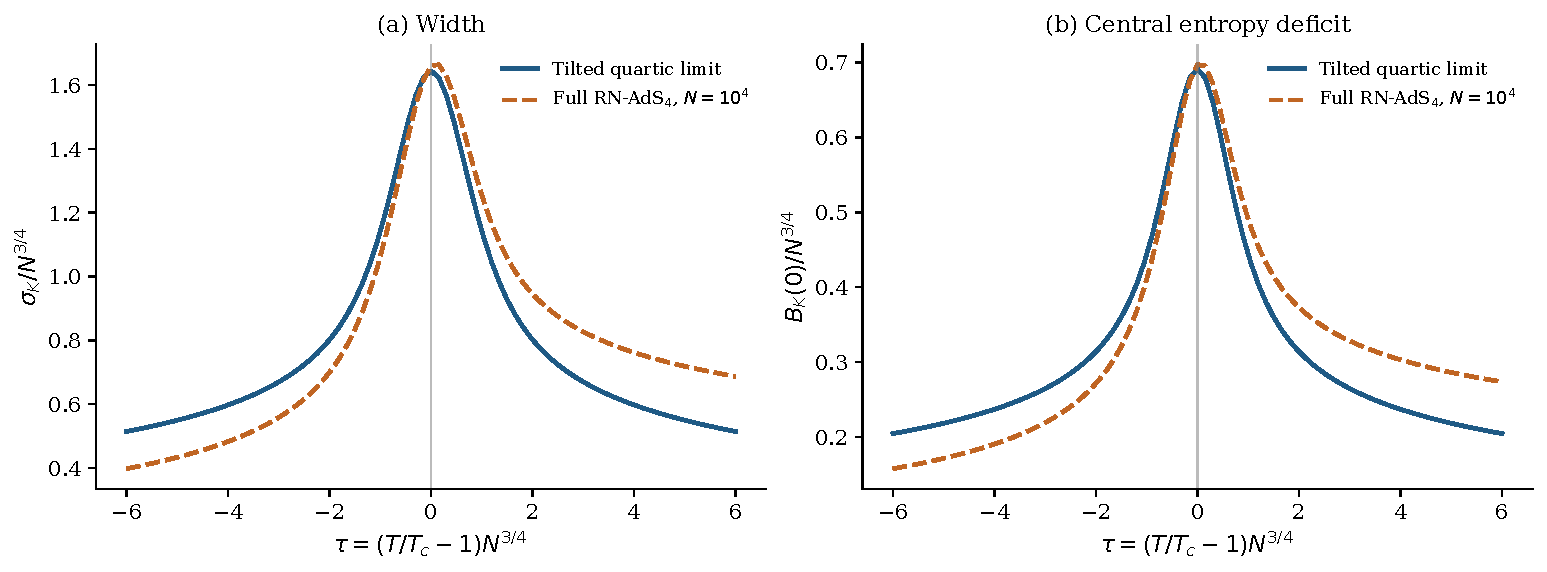
\includegraphics[width=\textwidth]{figures/output/jhep2_temperature.pdf}
 \caption{Temperature dependence within the critical finite-size
 window for four-dimensional RN--AdS.  The full canonical model
 at $N=10^4$ is compared with the quartic limiting law:
 (a)~the standard deviation $\sigma_K/N^{3/4}$;
 (b)~the central deficit $B_N(0)/N^{3/4}$.
 Both panels use the centered modular energy $K(E)$.
 The horizontal variable is $\tau=tN^{3/4}$, for which
 $h=2\sqrt2\,\tau$ when $d=3$.  The limiting width remains finite
 at $\tau=0$.  The finite-$N$ curve retains the asymmetry of the
 full action and measure.}
 \label{fig03:temperature}
\end{figure}

\subsection{An exact four-dimensional action}

In four bulk dimensions, $r_c=\ell/\sqrt6$, $q_c=\ell/6$, and
$N=\pi\ell^2/(6G)$.  The reduced mass and entropy are
\begin{equation}
 \frac{\beta_c M(R)}{N}=\frac{R^3}{4}
                 +\frac{3R}{2}+\frac{1}{4R},\qquad
 \frac{S(R)}{N}=R^2.
 \label{eq03:rn4_mass}
\end{equation}
Their difference factorizes exactly:
\begin{equation}
 \frac{I_c(R)}{N}=1+\frac{(R-1)^4}{4R},\qquad
 R\geq R_{\mathrm{ext}}
       =\sqrt{-1+\frac{2}{\sqrt3}}.
 \label{eq03:rn4_action}
\end{equation}
Thus the full canonical density used in the numerical calculations
is proportional to
\begin{equation}
 \left(\frac{3R^2}{4}+\frac32-\frac{1}{4R^2}\right)
 \exp\!\left[-\frac{N(R-1)^4}{4R}\right]\dd R
 \label{eq03:rn4_density}
\end{equation}
on this physical domain.  The factor in parentheses is
$\beta_c M_R'/N$ and vanishes at extremality.  No fit to a
critical exponent is required to evaluate this integral.

For comparison with \eqref{eq03:scales}, the variable
$y=N^{1/4}(R-1)$ has limiting density proportional to
$e^{-y^4/4}$, and $(S-\E S)/N^{3/4}$ tends to $2y$.
The resulting coefficients are
\begin{equation}
 \frac{\sigma_S}{N^{3/4}}\longrightarrow1.644357917\ldots,
 \qquad
 \frac{B_{S,N}(0)}{N^{3/4}}\longrightarrow0.691367339\ldots,
 \label{eq03:rn4_coefficients}
\end{equation}
where $B_{S,N}(0)=\tfrac12\E|S-\E S|$.  These are also the
limiting coefficients for $K$, although the two finite-$N$
distributions are distinct.  Table~\ref{tab03:convergence} and
figure~\ref{fig03:critical} evaluate the full measure rather than
only its quartic approximation.

\begin{table}[tbp]
 \centering
 \caption{Convergence of the four-dimensional critical canonical
 integral \eqref{eq03:rn4_density}.  Both columns use the
 thermodynamic entropy $S(E)=NR^2$ and are centered at its exact
 numerical mean.  The table does not substitute $S(E)$ for the
 finite-$N$ modular energy $K(E)$.}
 \label{tab03:convergence}
 \begin{adjustbox}{max width=\textwidth,center}
 \begin{tabular}{rcc}
 \toprule
 $N$ & $\sigma_S/N^{3/4}$ & $B_{S,N}(0)/N^{3/4}$ \\
 \midrule
 $10^2$ & $1.798150$ & $0.748514$ \\
 $10^3$ & $1.693747$ & $0.709601$ \\
 $10^4$ & $1.660051$ & $0.697147$ \\
 $10^5$ & $1.649328$ & $0.693196$ \\
 $10^6$ & $1.645930$ & $0.691946$ \\
 $\infty$ & $1.644358$ & $0.691367$ \\
 \bottomrule
 \end{tabular}
 \end{adjustbox}
\end{table}

\begin{figure}[tbp]
 \centering
 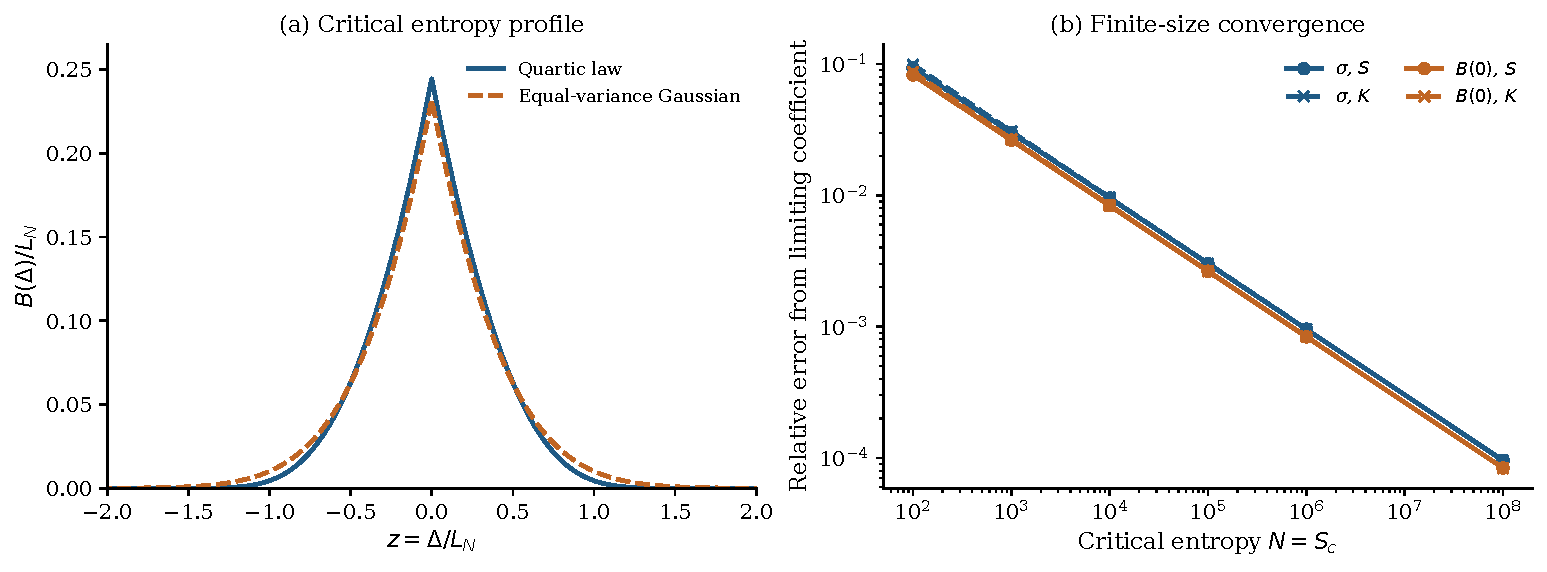
\includegraphics[width=\textwidth]{figures/output/jhep2_critical.pdf}
 \caption{Critical rounding and its finite-size convergence.
 (a)~The limiting deficit $B_N(\Delta)/L_N$ as a function of
 $z=\Delta/L_N$, given by \eqref{eq03:quartic_profile}, and a
 Gaussian with the same variance.
 (b)~Relative errors of the four-dimensional width and central
 deficit against their limiting coefficients in
 \eqref{eq03:rn4_coefficients}, computed separately for
 $S(E)$ and $K(E)$.  All finite-$N$ values use the full energy
 measure $e^{S(E)-\beta_c E}\dd E$ on the outer-horizon branch.}
 \label{fig03:critical}
\end{figure}

The exponent $3/4$ enters the entropy transition because the
fluctuating branch has a nonzero linear response to $R-1$ at the
critical point.  More generally, a generalized-entropy difference
whose derivative there is of order $N$ inherits this scale if its
fluctuations are described by the same canonical law.  If the
linear responses of the competing branches cancel, the difference
need not have an $N^{3/4}$ width.  An application to a specified
gravitational entanglement transition must therefore identify both
the probability measure and the coupling of its entropy difference
to the critical mode.

\section{Finite reservoirs and conserved energy}
\label{sec04:reservoir}

The canonical distribution in section~\ref{sec03:critical} describes a system coupled to a reservoir whose temperature does not change appreciably during an energy fluctuation. A finite reservoir changes both the distribution and the entropy difference relevant to a transition. In particular, fixing the total energy of a black hole and its radiation does not fix the black-hole energy. We first separate these two constraints and then determine the reservoir size required to retain the critical distribution.

\subsection{Energy exchange and the variance of an entropy difference}

Let the black hole and reservoir have entropies $S_B(E_B)$ and $S_R(E_R)$, with $E_B+E_R=E_{\mathrm{tot}}$. In a density-of-states approximation, their energy distribution is
\begin{equation}
 p(E_B)\,\dd E_B\propto
 \exp\!\left[S_B(E_B)+S_R(E_{\mathrm{tot}}-E_B)\right]\dd E_B.
 \label{eq04:energy_distribution}
\end{equation}
At a stationary point, $T_B=T_R=T$. Write $\epsilon=E_B-E_{B,*}$ and let $C_B$ and $C_R$ denote the heat capacities at this point, with all other conserved parameters held fixed. The entropy expansion is
\begin{equation}
 S_B(E_B)+S_R(E_R)
 =S_* -\frac{\epsilon^2}{2T^2}
 \left(\frac{1}{C_B}+\frac{1}{C_R}\right)+O(\epsilon^3).
 \label{eq04:entropy_hessian}
\end{equation}
Consequently, whenever the quadratic approximation controls the distribution,
\begin{equation}
 \Var E_B=T^2 C_{\mathrm{eff}},\qquad
 C_{\mathrm{eff}}=\left(C_B^{-1}+C_R^{-1}\right)^{-1}.
 \label{eq04:effective_capacity}
\end{equation}
For positive capacities this is the familiar harmonic combination appearing in the entanglement of a finite-energy chaotic system~\cite{murthysrednicki2019}. The condition for local stability is
\begin{equation}
 C_B^{-1}+C_R^{-1}>0.
 \label{eq04:stability}
\end{equation}
It is a condition on the combined system. A negative black-hole heat capacity is therefore compatible with local stability against energy exchange if $C_R>0$ and $C_R<|C_B|$. This local statement does not establish dominance over other phases.

To first order in the exchanged energy,
\begin{equation}
 \delta S_B=\frac{\epsilon}{T},\qquad
 \delta S_R=-\frac{\epsilon}{T}.
 \label{eq04:linear_entropies}
\end{equation}
Thus the entropy of either subsystem and the difference between them have different variances:
\begin{equation}
 \Var S_B\simeq C_{\mathrm{eff}},\qquad
 \Var(S_B-S_R)\simeq 4C_{\mathrm{eff}}.
 \label{eq04:gap_variance}
\end{equation}
The factor of four follows from the anticorrelation imposed by energy conservation. If the two competing entropy branches are $S_B$ and $S_R$, their leading averaged-minimum deficit at equal mean entropies is therefore
\begin{equation}
 B(0)\simeq \sqrt{\frac{2C_{\mathrm{eff}}}{\pi}}
 \label{eq04:gaussian_deficit}
\end{equation}
in the Gaussian regime. For $C_B=C_R=C$, this is $\sqrt{C/\pi}$, or $\sqrt{C_{\mathrm{tot}}/(2\pi)}$ with $C_{\mathrm{tot}}=2C$. The result agrees with the enhanced correction for an equal bipartition in the energy-eigenstate calculation of ref.~\cite{murthysrednicki2019}.

The total entropy, by contrast, is stationary at equilibrium: its fluctuation starts at second order in $\epsilon$. Appendix~\ref{app09:cost} gives the resulting gamma distribution of the entropy loss and explains why its variance is distinct from the subsystem variances in~\eqref{eq04:gap_variance}.

Equation~\eqref{eq04:gap_variance} is specific to this pair of branches. More generally, for branches $F_1(E_B,E_R)$ and $F_2(E_B,E_R)$, the coefficient multiplying $\epsilon$ is
\begin{equation}
 \left.(\partial_{E_B}-\partial_{E_R})(F_1-F_2)\right|_*.
 \label{eq04:general_branch_derivative}
\end{equation}
The variance relevant to the transition is the square of this coefficient times $\Var E_B$. A fluctuation shared by both branches can cancel from their difference. In particular, a heat-capacity singularity alone does not establish an enhanced entanglement correction.

Several ensemble limits can now be distinguished. The canonical variance of $S_B$ is recovered when $C_R/C_B\to\infty$, with $C_B>0$. If $C_B$ grows while $C_R$ is fixed, the reservoir limits the energy fluctuations; the Gaussian formula approaches $\Var S_B\simeq C_R$ only if the reservoir itself admits the required quadratic approximation. A genuinely small reservoir generally requires its full density of states. Fixing $E_B$ directly removes this classical energy fluctuation altogether. It does not remove the order-one Page correction inside an allowed energy sector, nor does it imply that every fixed-total-energy state has only order-one rounding.

\subsection{A reservoir coupled to the charged critical point}

At the critical point of section~\ref{sec03:critical}, the quadratic term in the canonical black-hole action vanishes. A finite reservoir restores a quadratic term whose competition with the quartic black-hole action can be computed explicitly.

Write $M_c=M(r_c)$ and $E_{R,c}=E_{\mathrm{tot}}-M_c$. Choose $E_{\mathrm{tot}}$ so that the reservoir has temperature $T_c$ at $E_B=M_c$. Let $\epsilon=E_B-M_c$ and assume that its heat capacity $C_R$ there is positive. Expanding its entropy gives
\begin{equation}
 S_R(E_{R,c}-\epsilon)
 =S_R(E_{R,c})-\frac{\epsilon}{T_c}
 -\frac{\epsilon^2}{2T_c^2 C_R}+\mathcal R_R(\epsilon).
 \label{eq04:reservoir_expansion}
\end{equation}
We first consider a finite limit of $L_N^2/(2C_R)$. Assume that $\mathcal R_R(T_cL_N X)=o(1)$ uniformly for bounded $X$, and that the allowed reservoir energies contain every bounded interval on this fluctuation scale for sufficiently large $N$.

Entropy moments require global tail control in addition to this local expansion. At the fluctuation scale $a_N$, define
\begin{equation}
 Y_N=\frac{\epsilon}{T_c a_N},\qquad
 Z_{R,N}=\frac{S_R(E_{R,c}-\epsilon)-S_R(E_{R,c})}{a_N}.
 \label{eq04:tail_variables}
\end{equation}
We require $Y_N^2$ to be uniformly integrable under the normalized composite distribution. For results involving reservoir entropy, we also require uniform integrability of $Z_{R,N}^2$. Here uniform integrability means, for example, $\lim_{A\to\infty}\sup_N\E[Y_N^2\boldsymbol{1}_{|Y_N|>A}]=0$. In the present finite-limit regime we take $a_N=L_N$. These conditions exclude rare remote regions that carry a vanishing probability but a finite or divergent entropy variance.

The local remainder condition holds, for example, for a smooth extensive reservoir with $C_R\asymp N^{3/2}$ and nonsingular intensive response functions: its cubic entropy term on this scale is $O(N^{-3/4})$. The tail conditions are separate assumptions; they do not follow from the local heat capacity.

The first law and the critical scaling give
\begin{equation}
 \frac{\epsilon}{T_c}=L_N X+o(L_N),\qquad
 L_N=(d-1)a_d^{-1/4}N^{3/4},
 \label{eq04:energy_critical_scale}
\end{equation}
where $X=(a_dN)^{1/4}(r/r_c-1)$ and $a_d=(d-1)(2d-3)/24$. Combining the canonical action with \eqref{eq04:reservoir_expansion} yields the limiting density
\begin{equation}
 p_u(X)=\frac{e^{-X^4-uX^2}}{Z_u},\qquad
 Z_u=\int_{\mathbb R}e^{-x^4-ux^2}\,\dd x,\qquad
 u=\lim_{N\to\infty}\frac{L_N^2}{2C_R}\geq0.
 \label{eq04:reservoir_quartic}
\end{equation}
The local expansion and tightness give this normalized limiting law. The energy-moment condition also controls black-hole entropy moments: on the RN outer-horizon family, $|S_B-S_c|/[\beta_c|E_B-M_c|]$ is bounded uniformly in $N$, extends continuously through $r_c$, and tends to zero at large radius. Local linearization and uniform integrability therefore give the leading entropy width and central averaged-minimum deficit for the fluctuating black-hole branch,
\begin{equation}
 \sigma_B\sim L_N\sqrt{\langle X^2\rangle_u},\qquad
 B_B(0)\sim\frac{L_N}{2}\langle |X|\rangle_u.
 \label{eq04:reservoir_observables}
\end{equation}
The subscript on $B_B$ specifies that the other branch is deterministic at the mean black-hole entropy. For two entropy branches exchanged under the fixed-total-energy constraint, the leading fluctuating difference is $2L_NX$, and both the width and central deficit are twice those in \eqref{eq04:reservoir_observables}.

The reservoir must therefore satisfy $C_R\gg N^{3/2}$ to reproduce the unrestricted canonical critical law. If $C_R\asymp N^{3/2}$, both terms in \eqref{eq04:reservoir_quartic} survive. In the reservoir-limited double limit $C_R\to\infty$ with $C_R\ll N^{3/2}$, we impose the same moment conditions separately at the narrower scale $a_N=\sqrt{C_R}$, together with $\mathcal R_R(T_c\sqrt{C_R}\,y)=o(1)$ uniformly on bounded $y$ and an allowed energy range containing those intervals. Then $\epsilon/(T_c\sqrt{C_R})$ tends to a standard Gaussian, and
\begin{equation}
 \sigma_B\sim\sqrt{C_R},\qquad
 B_B(0)\sim\sqrt{\frac{C_R}{2\pi}},
 \label{eq04:reservoir_limited}
\end{equation}
The quartic black-hole action on this narrower scale is $O(C_R^2/N^3)=o(1)$, whereas the reservoir contributes $y^2/2$. The moment conditions at this scale justify the Gaussian entropy moments in~\eqref{eq04:reservoir_limited}; conditions only on the broader canonical scale would not suffice. The crossover capacity $N^{3/2}$ is the square of the canonical critical entropy width. In a regular phase the corresponding scale is only order $N$, and an asymptotically unperturbed canonical variance requires $C_R/C_B\to\infty$.

In four bulk dimensions, the alternative variable $y=N^{1/4}(r/r_c-1)$ makes the coefficients particularly simple. With $b=C_R/N^{3/2}$,
\begin{equation}
 p_b(y)\propto\exp\!\left(-\frac{y^4}{4}-\frac{2y^2}{b}\right),\qquad
 \frac{\sigma_B}{N^{3/4}}\longrightarrow
 2\sqrt{\langle y^2\rangle_b}.
 \label{eq04:four_dimensional_bath}
\end{equation}
Figure~\ref{fig04:reservoir} displays this interpolation and the associated ratio $B_B(0)/\sigma_B$. That ratio approaches $1/\sqrt{2\pi}$ in the Gaussian limit and $2^{-5/4}$ in the canonical quartic limit. Thus the reservoir changes the shape of the entropy crossover as well as its width.

\begin{figure}[tbp]
 \centering
 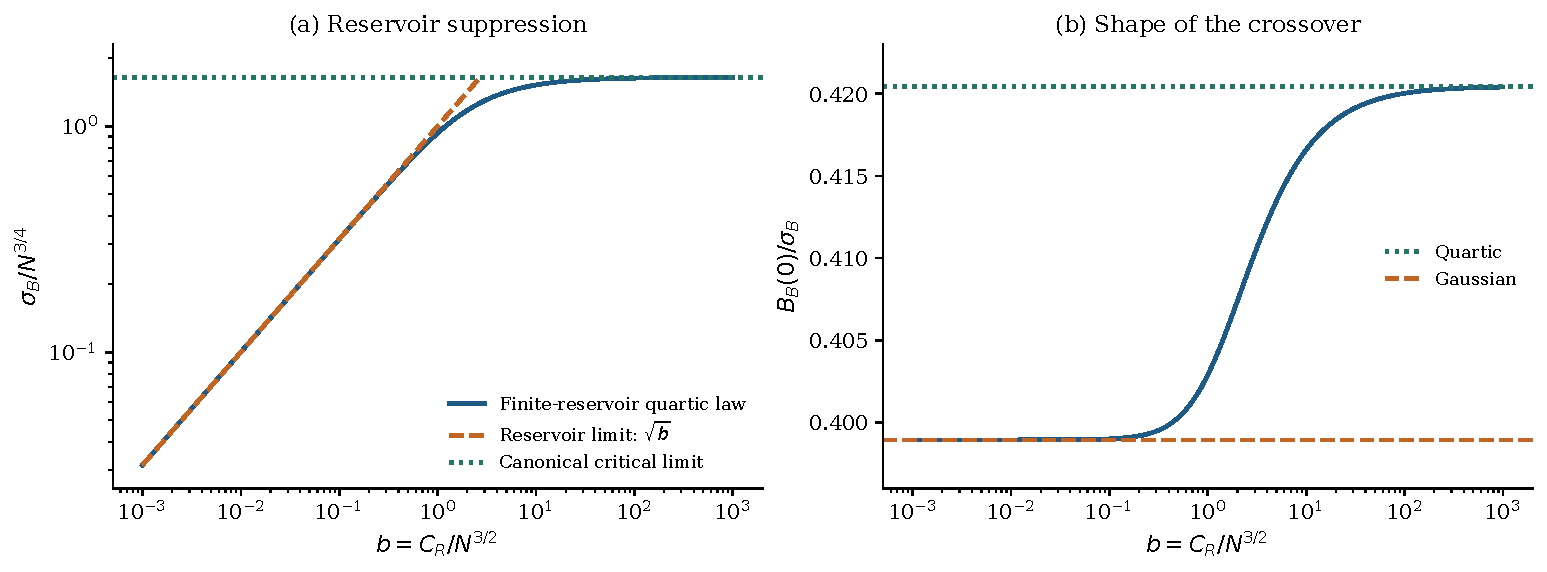
\includegraphics[width=\textwidth]{figures/output/jhep2_reservoir.pdf}
 \caption{Finite-reservoir modification of the four-dimensional charged critical distribution, computed from the normalized density in \eqref{eq04:four_dimensional_bath}. Left: the black-hole entropy width as a function of $b=C_R/N^{3/2}$, with the small-$b$ asymptote $\sigma_B/N^{3/4}\sim\sqrt b$ and the canonical quartic limit. Right: the ratio of the central deficit to this width, interpolating between Gaussian and quartic values. For the difference of two entropies exchanged under a fixed-total-energy constraint, both the leading width and deficit are twice their black-hole-branch values.}
 \label{fig04:reservoir}
\end{figure}

\subsection{Additional constraints and energy sectors}

The Gaussian calculation extends to several conserved quantities without assigning an independent variance to each entropy branch. Let $z$ be a vector of centered Gaussian fluctuations with positive-definite covariance $\Sigma$, and impose linear constraints $Az=0$, with $A$ of full row rank. The conditional covariance is
\begin{equation}
 \Sigma_{\mathrm{cond}}
 =\Sigma-\Sigma A^{\mathsf T}
 (A\Sigma A^{\mathsf T})^{-1}A\Sigma.
 \label{eq04:conditional_covariance}
\end{equation}
It follows by completing the square in the joint Gaussian density, or by subtracting the linear regression of $z$ on $Az$. For an entropy difference whose linearization is $v^{\mathsf T}z$, the variance is $v^{\mathsf T}\Sigma_{\mathrm{cond}}v$. This formula applies when the unconstrained Gaussian exists. A negative-capacity subsystem instead requires direct analysis of the constrained entropy Hessian, as in \eqref{eq04:entropy_hessian}.

Finally, energy conservation can also change the Hilbert-space structure. Suppose the radiation and black-hole spaces decompose into mutually orthogonal energy sectors and a pure state has the form
\begin{equation}
 |\Psi\rangle=\sum_\alpha\sqrt{p_\alpha}\,|\psi_\alpha\rangle,
 \qquad
 |\psi_\alpha\rangle\in
 \mathcal H_{R,\alpha}\otimes\mathcal H_{B,\alpha}.
 \label{eq04:energy_sector_state}
\end{equation}
Tracing out the black hole gives a direct sum, and hence the exact identity
\begin{equation}
 S(\rho_R)=H(p)+\sum_\alpha p_\alpha S(\rho_{R,\alpha}),
 \qquad H(p)=-\sum_\alpha p_\alpha\log p_\alpha.
 \label{eq04:block_entropy}
\end{equation}
An averaged minimum can approximate the entropies within sectors, but the sector entropy $H(p)$ must also be retained at the accuracy where it contributes. Energy-eigenstate calculations similarly organize the entropy by the energy assigned to each subsystem, with additional care for interactions and finite energy windows~\cite{murthysrednicki2019,dongwang2020}. This differs from the canonically weighted random-state model of section~\ref{sec02:model}. In particular, the spectral correction for energy sectors cannot be inferred by transferring the planar correction of that model without a separate calculation.

\section{Spinodals and phase coexistence}
\label{sec05:phases}

The charged critical point is not the only place where a black-hole heat capacity becomes large. A spinodal and a first-order coexistence point nevertheless require different probability distributions. Schwarzschild--AdS provides a direct way to separate them, because the minimum black-hole temperature and the Hawking--Page temperature are distinct.

\subsection{The minimum temperature of Schwarzschild--AdS}

For a spherical Schwarzschild--AdS black hole in $d+1$ dimensions,
\begin{equation}
 S(r)=\frac{\Omega_{d-1}r^{d-1}}{4G},\qquad
 T_H(r)=\frac{d r^2+(d-2)\ell^2}{4\pi\ell^2r},\qquad
 C_\ell(r)=(d-1)S(r)
 \frac{d r^2+(d-2)\ell^2}{d r^2-(d-2)\ell^2}.
 \label{eq05:schwarzschild_thermodynamics}
\end{equation}
The temperature has a minimum at
\begin{equation}
 r_0=\ell\sqrt{\frac{d-2}{d}},\qquad
 T_0=\frac{\sqrt{d(d-2)}}{2\pi\ell}.
 \label{eq05:minimum_temperature}
\end{equation}
The large-black-hole branch has positive heat capacity for $r>r_0$; the smaller branch has negative heat capacity. Their merger at $T_0$ is a spinodal, the endpoint of local stability of the large-black-hole saddle.

Set $N_0=S(r_0)$, $x=r/r_0-1$, and $t_0=(T-T_0)/T_0$. The exact ratio $T_H/T_0=\tfrac12[(1+x)+(1+x)^{-1}]$ and the first law imply
\begin{equation}
 I'(x)=S'(x)\left(\frac{T_H(x)}{T}-1\right),
 \qquad I=\frac{M}{T}-S.
 \label{eq05:spinodal_action_derivative}
\end{equation}
Consequently, in a neighborhood of the spinodal,
\begin{equation}
 I(x)-I(0)
 =(d-1)N_0\left(\frac{x^3}{6}-t_0x\right)
 +O\!\left(N_0[x^4+|t_0|x^2+t_0^2|x|]\right).
 \label{eq05:cubic_action}
\end{equation}
For small positive $t_0$, the two stationary radii satisfy $x_\pm=\pm\sqrt{2t_0}+O(t_0)$, with the plus sign denoting the locally stable saddle. The entropy width obtained by a quadratic expansion about this saddle is
\begin{equation}
 \sigma_S\simeq\sqrt{C_\ell}
 \sim\sqrt{(d-1)N_0}\,(2t_0)^{-1/4}.
 \label{eq05:spinodal_gaussian_width}
\end{equation}
Its validity requires the radial fluctuation to remain small compared with the distance to the unstable saddle. Equivalently, the action barrier
\begin{equation}
 I(x_-)-I(x_+)
 \sim\frac{4\sqrt2}{3}(d-1)N_0t_0^{3/2}
 \label{eq05:spinodal_barrier}
\end{equation}
must be large. Both conditions give
\begin{equation}
 t_0\gg N_0^{-2/3}.
 \label{eq05:spinodal_validity}
\end{equation}
The divergent Gaussian width cannot be extrapolated through this range boundary. In particular, equating \eqref{eq05:spinodal_gaussian_width} to the order-$N_0$ entropy would require $t_0\asymp N_0^{-2}$, already far outside its regime of validity.

The cubic normal form also explains why the critical-point argument does not carry over directly. The function $\exp[-(d-1)y^3/6]$ is not integrable on the full real line. If one imposes a hard restriction to the large-black-hole basin, then $t_0=\tau_0N_0^{-2/3}$ and $x=N_0^{-1/3}y$ give the formal conditioned density
\begin{equation}
 p_{\tau_0}^{\mathrm{basin}}(y)\propto
 \exp\!\left[-(d-1)\left(\frac{y^3}{6}-\tau_0y\right)\right],
 \qquad y\geq-\sqrt{2\tau_0},\quad \tau_0\geq0.
 \label{eq05:conditioned_spinodal}
\end{equation}
It produces entropy fluctuations of order $N_0^{2/3}$. This is a statement about the specified basin restriction. A dynamical quasistationary distribution need not equal \eqref{eq05:conditioned_spinodal}, and the vanishing barrier prevents a general inference of a long-lived metastable state at $\tau_0=0$. We therefore do not assign the conditioned scale to the equilibrium canonical Page transition.

\subsection{The Hawking--Page mixture}

The Hawking--Page transition occurs instead at~\cite{hawkingpage1983}
\begin{equation}
 r_{\mathrm{HP}}=\ell,\qquad
 T_{\mathrm{HP}}=\frac{d-1}{2\pi\ell}>T_0.
 \label{eq05:hawking_page_temperature}
\end{equation}
At this point the classical free energies of thermal AdS and the large black hole coincide. Between $T_0$ and $T_{\mathrm{HP}}$, the large black hole is only metastable in the canonical ensemble that includes thermal AdS. At $T_{\mathrm{HP}}$, its conditional heat capacity is finite:
\begin{equation}
 C_{\ell,\mathrm{HP}}=(d-1)^2 S_{\mathrm{HP}}.
 \label{eq05:hp_capacity}
\end{equation}
Its within-phase entropy width is therefore of order $S_{\mathrm{HP}}^{1/2}$, not divergent.

For an equilibrium model containing both phases, the additional fluctuation is the choice of phase. Let $w$ be the probability of the black-hole phase, and let $\mu_B,\mu_A$ and $V_B,V_A$ denote the conditional means and variances of a chosen random variable in the black-hole and thermal-AdS phases. The law of total variance gives
\begin{equation}
 V=wV_B+(1-w)V_A+w(1-w)(\mu_B-\mu_A)^2.
 \label{eq05:mixture_variance}
\end{equation}
For canonical modular energy $K=\beta E+\log Z$, the mean separation at coexistence is $\beta\Delta M$ to leading order. The equality of free energies gives $\beta\Delta M=\Delta S\asymp S_{\mathrm{HP}}$. Thus a mixture with both weights of order one has an order-$S_{\mathrm{HP}}$ width. The dominant term in \eqref{eq05:mixture_variance} is the separation of the phases, and the distribution is bimodal rather than a Gaussian with a large variance.

The temperature range supporting both phases follows from their partition functions. Write $Z_i=A_i e^{-I_i}$, where $i=A,B$ and the factors $A_i$ include fluctuations around each phase. With $\theta=(T-T_{\mathrm{HP}})/T_{\mathrm{HP}}$,
\begin{equation}
 I_B-I_A=-\Delta S\,\theta+O(S_{\mathrm{HP}}\theta^2),\qquad
 w=\frac{1}{1+\exp\!\left[I_B-I_A-\log(A_B/A_A)\right]}.
 \label{eq05:phase_weight}
\end{equation}
The coexistence window has relative temperature width $O(S_{\mathrm{HP}}^{-1})$. A prefactor ratio whose logarithm is $O(\log S_{\mathrm{HP}})$ shifts the equal-weight temperature by $O(\log S_{\mathrm{HP}}/S_{\mathrm{HP}})$, without changing that width. The classical equality of actions should not be confused with exact equal probabilities at finite entropy.

The entropy model of section~\ref{sec02:model} can be applied to this mixture by retaining both components of the modular-energy distribution. For illustration, two equally weighted narrow components separated by $D$ give a central deficit $B(0)=D/4$ at leading order. The crossover has two changes of slope separated by $D$; replacing the mixture by a Gaussian would lose this structure. A gravitational application requires more: the candidate generalized-entropy surfaces must be specified in each phase, and the entropy of the phase mixture must be treated consistently. Equation~\eqref{eq05:mixture_variance} alone does not supply those ingredients.

\subsection{Charged coexistence below the critical point}

The small/large charged-black-hole transition provides a further distinction between a first-order line and its critical endpoint~\cite{chamblin1999,kubiznakmann2012}. In four bulk dimensions its coexistence curve is known analytically~\cite{spallucci2013}; the following radius-ratio parametrization makes the equality of free energies explicit. For this paragraph use the conventional geometric units $G=1$, take the metric charge parameter $q>0$ without loss of generality, and define $P=3/(8\pi\ell^2)$. The temperature and Gibbs free energy at fixed $P,q$ are
\begin{equation}
 T(r)=\frac{1}{4\pi r}\left(1+8\pi Pr^2-\frac{q^2}{r^2}\right),
 \qquad
 \mathcal G(r)=\frac{r}{4}\left(1-\frac{8\pi Pr^2}{3}
 +\frac{3q^2}{r^2}\right).
 \label{eq05:rn_gibbs}
\end{equation}
If $\lambda=r_s/r_l\in(0,1]$ and $D_\lambda=\lambda^2+4\lambda+1$, equal temperatures and Gibbs free energies are satisfied by
\begin{align}
 r_s&=q\sqrt{D_\lambda}, & r_l&=\frac{q\sqrt{D_\lambda}}{\lambda},\nonumber\\
 P&=\frac{3\lambda^2}{8\pi q^2D_\lambda^2}, &
 T&=\frac{\lambda(1+\lambda)}{\pi qD_\lambda^{3/2}}.
 \label{eq05:rn_coexistence_parametric}
\end{align}
Substitution into \eqref{eq05:rn_gibbs} verifies both equalities directly. With $p=P/P_c$ and $\vartheta=T/T_c$,
\begin{equation}
 p=\frac{36\lambda^2}{D_\lambda^2},\qquad
 \vartheta=\frac{3\sqrt6\lambda(1+\lambda)}{D_\lambda^{3/2}},\qquad
 \vartheta^2=\frac{p(3-\sqrt p)}{2}.
 \label{eq05:rn_coexistence_reduced}
\end{equation}
Figure~\ref{fig05:phases} compares these phase boundaries. The first-order line has two distinct stable saddles. At its endpoint the separation vanishes and the quartic distribution of section~\ref{sec03:critical} replaces the two-saddle approximation. The coexistence curve determines the relative saddle locations and actions; it does not determine an entanglement transition without a state and entropy prescription. Island calculations for charged AdS black holes address that additional geometric problem~\cite{lin2024}.

\begin{figure}[tbp]
 \centering
 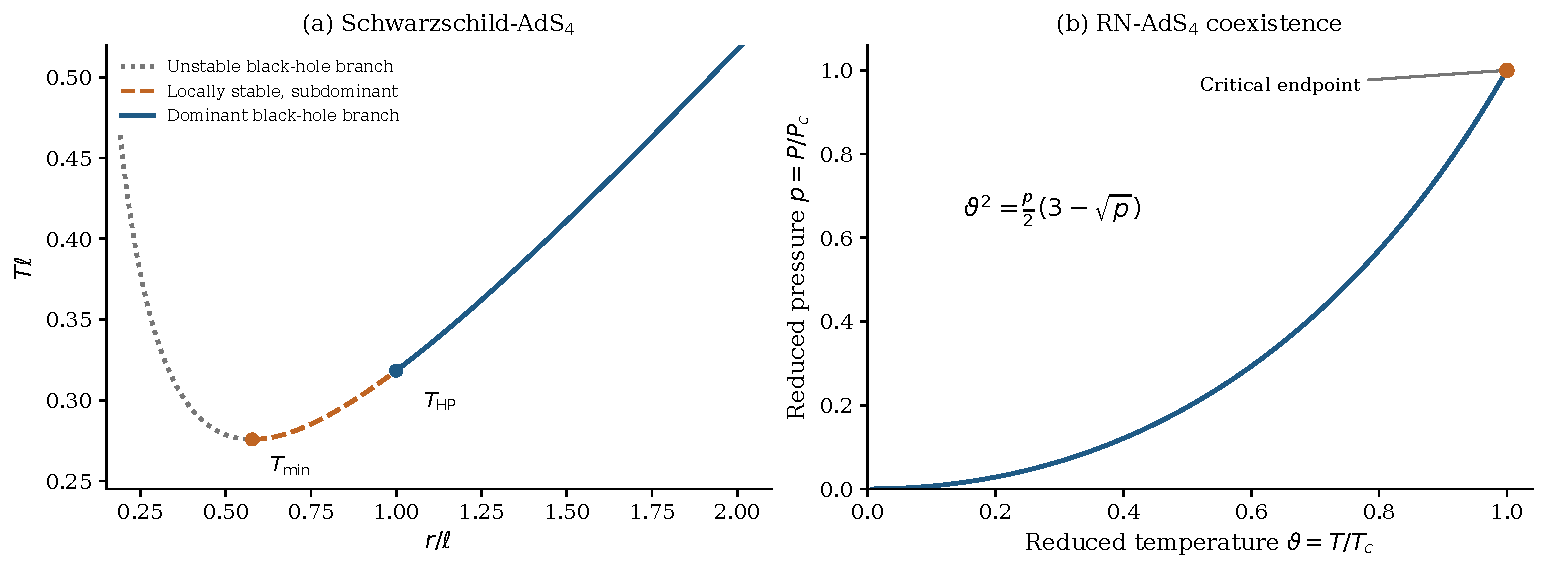
\includegraphics[width=\textwidth]{figures/output/jhep2_phases.pdf}
 \caption{Distinct thermodynamic mechanisms in four bulk dimensions. Left: the Schwarzschild--AdS temperature curve separates the merger of black-hole saddles at $T_0$ from coexistence with thermal AdS at $T_{\mathrm{HP}}$. The locally stable branch between these temperatures is metastable when thermal AdS is included. Right: the charged small/large-black-hole coexistence curve, computed from the equal-temperature, equal-free-energy solution \eqref{eq05:rn_coexistence_parametric}, terminates at the charged critical point.}
 \label{fig05:phases}
\end{figure}

The resulting hierarchy is conditional on the stated ensemble. In an ordinary stable phase, the width scales as the square root of the black-hole entropy. The charged canonical critical point instead gives $N^{3/4}$, while coexistence gives a width proportional to the latent entropy when both phase weights remain finite. The formal $N_0^{2/3}$ spinodal scale additionally requires a restriction to a metastable basin. These powers describe different distributions and cannot be inferred from one divergent Gaussian heat-capacity formula.

\section{Corrections away from criticality}
\label{sec06:cumulants}

Away from critical points and coexistence, a single stable canonical saddle produces Gaussian fluctuations at leading order. The first corrections depend on which fluctuating observable is used. This matters even when the leading entropy variance equals the heat capacity: the thermodynamic entropy $S(E)$ is nonlinear in energy, whereas the canonical modular energy $K(E)$ is affine.

\subsection{Two cumulant formulae}

Let $S_{\mathrm{eq}}(T)=S(E_*(T))$ denote the entropy at the nondegenerate saddle $S'(E_*)=1/T$, and let
\begin{equation}
 C(T)=\frac{\dd E_*}{\dd T}=T\frac{\dd S_{\mathrm{eq}}}{\dd T}.
 \label{eq06:saddle_capacity}
\end{equation}
All other thermodynamic variables are held fixed. Suppose the system is extensive in a large parameter $N$, the saddle remains separated from boundaries and other saddles, and its derivatives admit the usual regular Laplace expansion. In the density model~\eqref{eq02:density_of_states}, the leading extensive cumulants of $S(E)$ are
\begin{equation}
 \kappa_n[S(E)]
 =T^{n-1}\frac{\dd^{n-1}S_{\mathrm{eq}}}{\dd T^{n-1}}+O(1),
 \qquad n\geq2.
 \label{eq06:entropy_cumulants}
\end{equation}
The remainder here presumes a smooth, regular prefactor; it is not a formula at a degenerate saddle. To derive~\eqref{eq06:entropy_cumulants}, introduce a source $\lambda$ for $S(E)$. The tilted exponent is $(1+\lambda)S(E)-\beta E$, and its saddle is $E_*(T(1+\lambda))$. Differentiating its stationary value once with respect to $\lambda$ gives $S_{\mathrm{eq}}(T(1+\lambda))$; further derivatives give the displayed result. In particular,
\begin{align}
 \kappa_2[S]&=C+O(1),\nonumber\\
 \kappa_3[S]&=TC'-C+O(1),\nonumber\\
 \kappa_4[S]&=T^2C''-2TC'+2C+O(1),
 \label{eq06:entropy_cumulants_explicit}
\end{align}
where primes denote temperature derivatives.

For $K=\beta E+\log Z$, no saddle approximation is needed. Let $C_{\mathrm{can}}=\dd\E E/\dd T$ be the exact canonical heat capacity of the model. The cumulant generating function gives
\begin{equation}
 \kappa_n[K]=(-\beta)^n\partial_\beta^n\log Z,
 \qquad n\geq2,
 \label{eq06:modular_cumulants}
\end{equation}
and therefore
\begin{align}
 \kappa_2[K]&=C_{\mathrm{can}},\nonumber\\
 \kappa_3[K]&=TC_{\mathrm{can}}'+2C_{\mathrm{can}},\nonumber\\
 \kappa_4[K]&=T^2C_{\mathrm{can}}''+6TC_{\mathrm{can}}'+6C_{\mathrm{can}}.
 \label{eq06:modular_cumulants_explicit}
\end{align}
The leading terms of $C_{\mathrm{can}}$ and $C$ agree under the preceding saddle assumptions. Their common variance does not make the higher cumulants interchangeable.

As a simple example, suppose $S_{\mathrm{eq}}=A T^m$, with $A>0$ large and $m>0$ fixed. This includes the leading large-radius AdS equation of state with $m=d-1$. At leading extensive order,
\begin{equation}
 \begin{aligned}
 \kappa_2[S]&=mS_{\mathrm{eq}},&
 \kappa_3[S]&=m(m-1)S_{\mathrm{eq}},&
 \kappa_4[S]&=m(m-1)(m-2)S_{\mathrm{eq}},\\
 \kappa_2[K]&=mS_{\mathrm{eq}},&
 \kappa_3[K]&=m(m+2)S_{\mathrm{eq}},&
 \kappa_4[K]&=m(m+2)(m+3)S_{\mathrm{eq}}.
 \end{aligned}
 \label{eq06:power_law_cumulants}
\end{equation}
For instance, $m=2$ gives vanishing leading fourth cumulant for $S(E)$ but a nonzero leading fourth cumulant for $K(E)$. The equality of their broad Gaussian limits is consistent with this difference: their standardized third and fourth cumulants still vanish as $N^{-1/2}$ and $N^{-1}$, respectively.

\subsection{Integrating the Edgeworth expansion}

Let $\xi$ be the centered entropy fluctuation of interest, with its \emph{actual} standard deviation $\sigma$, standardized cumulants
\begin{equation}
 \gamma_1=\frac{\kappa_3[\xi]}{\sigma^3},\qquad
 \gamma_2=\frac{\kappa_4[\xi]}{\sigma^4},
 \label{eq06:standardized}
\end{equation}
and a regular density expansion about a Gaussian. For a noncritical extensive family, $\gamma_1=O(N^{-1/2})$ and $\gamma_2=O(N^{-1})$. To this order the density of $Y=\xi/\sigma$ is
\begin{equation}
 p_Y(y)=\phi(y)\left[
 1+\frac{\gamma_1}{6}H_3(y)
 +\frac{\gamma_2}{24}H_4(y)
 +\frac{\gamma_1^2}{72}H_6(y)\right]+r_N(y),
 \label{eq06:edgeworth_density}
\end{equation}
where $H_n(y)=(-1)^n\phi(y)^{-1}\dd^n\phi(y)/\dd y^n$ are the probabilists' Hermite polynomials. To use this expansion for an entropy expectation, one needs an integrated remainder bound, not just pointwise convergence of the density. For bounded $z=\Delta/\sigma$, the condition
\begin{equation}
 \int_{\mathbb R}(1+|y|)|r_N(y)|\,\dd y=o(N^{-1})
 \label{eq06:edgeworth_remainder}
\end{equation}
is sufficient for the remainder below to be $o(\sigma/N)$. Such a bound is an additional regularity assumption on the noncritical family.

Two integrations by parts give
\begin{equation}
 \int_{\mathbb R}\min(z,y)\phi(y)H_n(y)\,\dd y
 =-\phi(z)H_{n-2}(z),\qquad n\geq2.
 \label{eq06:hermite_integral}
\end{equation}
Thus the entropy correction contains Hermite polynomials of two degrees lower than the density correction:
\begin{equation}
 M(\Delta)=M_{\mathrm G}(\Delta)
 -\sigma\phi(z)\left[
 \frac{\gamma_1}{6}H_1(z)
 +\frac{\gamma_2}{24}H_2(z)
 +\frac{\gamma_1^2}{72}H_4(z)\right]
 +o(\sigma/N).
 \label{eq06:edgeworth_minimum}
\end{equation}
The squared-skewness term is the same order as the fourth-cumulant term and must be retained. At the crossing of the means,
\begin{equation}
 B(0)=\frac{\sigma}{\sqrt{2\pi}}
 \left[1+\frac{\gamma_1^2-\gamma_2}{24}
 +o(N^{-1})\right].
 \label{eq06:edgeworth_center}
\end{equation}
The first-order skewness correction vanishes there. Away from the center it is generally of order one, because $\sigma\gamma_1=O(1)$.

In the power-law example of~\eqref{eq06:power_law_cumulants}, the leading entropy-variable cumulants give
\begin{equation}
 \frac{\gamma_1^2-\gamma_2}{24}
 =\frac{m-1}{24mS_{\mathrm{eq}}}+O(S_{\mathrm{eq}}^{-2}),
 \label{eq06:power_law_entropy_correction}
\end{equation}
whereas the modular-energy cumulants give $-(m+2)/(24mS_{\mathrm{eq}})+O(S_{\mathrm{eq}}^{-2})$. This sign difference is a direct consequence of using different random variables. In both cases an order-one correction to the variance itself changes $B(0)$ at the same absolute order as the displayed non-Gaussian term. Replacing the actual $\sigma$ in~\eqref{eq06:edgeworth_center} by its leading saddle value therefore loses part of that order.

Equations~\eqref{eq06:edgeworth_minimum}--\eqref{eq06:edgeworth_center} concern the averaged minimum. They neither supply an order-one gravitational correction nor replace the planar correction in Proposition~\ref{prop02:spreading}. For the canonical random-state model, one must use the cumulants of $K$, retain the specified diagonal kernel if that accuracy is sought, and distinguish its entropy from $S_{\mathrm{planar}}$. At the charged critical point the standardized cumulants do not vanish, and the quartic law of Section~\ref{sec03:critical} must be used directly.

\section{Discussion}
\label{sec07:discussion}

The charged critical point admits a controlled entropy crossover after the Gaussian approximation has failed. Within the Reissner--Nordstr\"om--AdS density-of-states model, the quartic saddle determines both the $S_c^{3/4}$ scale and the limiting shape. The regular examples, critical calculation, and finite-reservoir analysis identify how that result depends on thermodynamic stability, the preparation of the state, and the entropy observable. We now compare these dependencies and their implications for gravitational entropy transitions.

\subsection{Distinct mechanisms of finite-size rounding}
\label{sec07:regimes}

In a regular canonical phase, the entropy fluctuation is the linear response to an approximately Gaussian energy fluctuation. Its standard deviation is $\sqrt C$ to leading order. The large-radius AdS relation $C\simeq(d-1)S$ then fixes the coefficient, as illustrated in section~\ref{sec10:regular}. The square-root law follows from a nondegenerate extensive saddle; the equation of state supplies the dimensional dependence. The exact finite-radius expression and the BTZ example show which parts of that relation persist beyond the large-radius approximation.

At the charged endpoint, the disappearance of the quadratic and cubic terms changes the radial scale from $N^{-1/2}$ to $N^{-1/4}$. Since the entropy has a nonzero linear derivative of order $N$, its width becomes $N^{3/4}$. The resulting correction is enhanced but still subextensive: its ratio to $N$ vanishes as $N^{-1/4}$. First-order coexistence has a different origin. There the phase label fluctuates between two components whose means are separated extensively. A mixture with finite weights can retain an extensive entropy deficit, even though the distribution within either phase remains narrow. Table~\ref{tab07:regimes} collects the scales and their distinct probability distributions.

\begin{table}[tbp]
 \centering
 \caption{Entropy standard deviations in the ensembles specified in the text. The first three rows refer to a single fluctuating entropy branch, or to canonical $K$ where appropriate. A general branch difference also requires its response coefficient. Here $S_*$ is a regular saddle entropy, $N=S_c$, $N_0=S(r_0)$, and $S_{\mathrm{HP}}$ is the Hawking--Page black-hole entropy.}
 \label{tab07:regimes}
 \begin{adjustbox}{max width=\textwidth,center}
 \begin{tabular}{p{0.21\textwidth}p{0.17\textwidth}p{0.52\textwidth}}
 \toprule
 Regime & Width & Distribution and conditions \\
 \midrule
 Regular canonical phase & $O(S_*^{1/2})$ & Gaussian; a single nondegenerate saddle with $C\asymp S_*$ and controlled tails. \\[3pt]
 Charged critical point & $O(N^{3/4})$ & Quartic; critical charge and $|T-T_c|/T_c=O(N^{-3/4})$, with an effectively infinite reservoir. \\[3pt]
 Reservoir-limited critical point & $\sim\sqrt{C_R}$ & Gaussian when $1\ll C_R\ll N^{3/2}$, subject to the local expansion and moment conditions of section~\ref{sec04:reservoir}. \\[3pt]
 Hawking--Page mixture & $O(S_{\mathrm{HP}})$ & Two phases with nonvanishing weights and an extensive separation of their modular-energy means. \\[3pt]
 Conditioned spinodal & $O(N_0^{2/3})$ & Cubic law restricted to the prescribed large-black-hole basin; a metastable conditioning, not a canonical equilibrium prediction. \\
 \bottomrule
 \end{tabular}
 \end{adjustbox}
\end{table}

The profile contains information beyond its width. For example, the central ratio $B(0)/\sigma$ distinguishes the symmetric quartic law from a Gaussian of identical variance, while a two-phase mixture produces two separated changes of slope. Equation~\eqref{eq02:curvature} makes this distinction precise: varying the reference dimension at fixed thermodynamic state gives the density of the centered modular energy through the curvature of the leading averaged minimum. The integrated identities in appendix~\ref{app08:identities} recover its moments. These statements concern a scan that translates the entropy difference while holding its fluctuation law fixed. A temperature scan also changes that law and therefore requires the two-variable profile~\eqref{eq03:thermal_profile}.

\subsection{Modular fluctuations and the response of an entropy difference}
\label{sec07:response}

The modular-energy variance has a standard quantum-information interpretation. For a normalized density matrix $\rho$, with $\tr\rho^n$ twice differentiable near $n=1$, the capacity of entanglement is~\cite{deboer2019}
\begin{equation}
 C_{\mathrm{ent}}(\rho)
 =\tr\rho\bigl[-\log\rho-S(\rho)\bigr]^2
 =\left.\partial_n^2\log\tr\rho^n\right|_{n=1}.
 \label{eq07:capacity}
\end{equation}
For the canonical black-hole state $\rho_\beta=Z^{-1}e^{-\beta H}$, this is exactly $\Var K=\beta^2\Var E=C_{\mathrm{can}}$. Thus the critical law gives a finite capacity of order $N^{3/2}$ for this state, with the coefficient in~\eqref{eq03:width_deficit}. This is the capacity of the canonical input state, rather than a calculation of the capacity of the reference state after the random-state construction. The distinction between $K(E)$ and $S(E)$ in section~\ref{sec06:cumulants} also persists: equality of their leading broad limits does not identify all their cumulants.

For two fluctuating branches, the relevant response is that of their difference. Let $D_N=F_1-F_2$ denote a specified entropy difference and suppose its critical response has the form
\begin{equation}
 D_N-\E D_N=Nc_1(R-\E R)+\mathcal R_N,
 \qquad \E\mathcal R_N^2=o(N^{3/2}),
 \label{eq07:critical_response}
\end{equation}
where $c_1\neq0$ has a finite, nonzero limit. If $R$ has the canonical critical distribution of proposition~\ref{prop03:quartic}, its moment convergence gives
\begin{equation}
 \sigma_D\sim |c_1|a_d^{-1/4}N^{3/4}
 \sqrt{\frac{\Gamma(3/4)}{\Gamma(1/4)}}.
 \label{eq07:projected_width}
\end{equation}
At the crossing of the means, the averaged-minimum deficit for these branches has the same limiting ratio $B_D(0)/\sigma_D\to2^{-5/4}$. Equation~\eqref{eq07:critical_response} states both the response and the moment control needed for that inference. For the canonical model, $F_1=K$ and $F_2=s$ give $c_1=d-1$ at leading order. If the two responses cancel, the nonlinear terms and any other fluctuating modes determine the result; a heat-capacity singularity alone does not specify it.

This projection is also useful away from criticality. If $z$ denotes several regular thermodynamic fluctuations, $D-\E D\simeq v^{\mathsf T}z$ has variance $v^{\mathsf T}\Sigma v$, with $\Sigma=\Cov z$. Conserved quantities replace $\Sigma$ by the conditional covariance in~\eqref{eq04:conditional_covariance}. An extension allowing angular-momentum or charge exchange would therefore require the susceptibility matrix in the chosen ensemble, its stable or critical directions, and the response vector $v$. The scalar heat capacity at fixed angular momentum or charge supplies only one part of that calculation. In particular, a critical direction contributes an enhanced transition width only when the entropy difference has a nonzero component along it.

\subsection{Relation to fixed-area states and quantum extremal surfaces}
\label{sec07:gravity}

The geometric setting for this response calculation is the competition between extremal surfaces. The Ryu--Takayanagi prescription and its covariant extension select an area extremum homologous to the boundary region~\cite{ryutakayanagi2006,hubeny2007}. The quantum extremal surface prescription replaces area by generalized entropy~\cite{engelhardtwall2015}. For candidate surfaces $\gamma_i$, the two branch values schematically take the form
\begin{equation}
 F_i=S_{\mathrm{gen}}(\gamma_i)
 =\frac{A(\gamma_i)}{4G}+S_{\mathrm{bulk}}(\gamma_i),
 \qquad D=F_1-F_2,
 \label{eq07:generalized_difference}
\end{equation}
with the area and bulk entropy combined in a consistent renormalization prescription. The response in~\eqref{eq07:critical_response} would then include the change of each surface and of the associated bulk state as the thermodynamic geometry fluctuates.

Fixed-area states provide a way to organize those fluctuations. Dong, Harlow and Marolf showed that projecting appropriate semiclassical states onto a definite extremal-surface area yields a flat entanglement spectrum at leading order in $1/G$~\cite{dong2019}. Akers and Rath obtained the corresponding maximal-entanglement condition within area eigenspaces from the quantum-error-correction description~\cite{akers2019}. These results separate the spectrum within a fixed geometric sector from the weights assigned to different sectors. Marolf, Wang and Wang subsequently used joint fixed-area fluctuations and a diagonal approximation to study enhanced corrections at entropy transitions~\cite{marolfwangwang2020}; Dong and Wang derived an enhanced correction by including replica saddles in a chaotic holographic example~\cite{dongwang2020}. In this setting the covariance of the two areas, and of their bulk-entropy corrections, is essential. Replacing it by two independent copies of a black-hole heat capacity would generally give a different entropy difference.

The thermodynamic calculation here supplies a candidate non-Gaussian law for one critical collective mode. To obtain a gravitational application, one can first identify the two quantum extremal surfaces in a specified state, calculate their difference along the charged family, and test~\eqref{eq07:critical_response}. One must also establish that the state samples the critical mode with the assumed measure and that other saddles or charged-matter instabilities do not dominate. If these conditions hold and the branch-averaging prescription is valid at the enhanced order, the quartic profile follows without replacing the critical mode by a Gaussian. Studies of islands in charged AdS geometries address the required surface competition~\cite{lin2024}; the fluctuation and state-preparation analysis is the complementary ingredient.

Replica-wormhole calculations establish the island mechanism for the entropy of Hawking radiation in concrete gravitational models~\cite{penington2020,almheiri2020,pssy2022}; ref.~\cite{almheirietal2021} reviews the relation among these constructions. They motivate comparing competing generalized entropies, while the treatment of fluctuations depends on the state and replica calculation. Leading spectral flatness within a fixed-area sector does not by itself determine the order-one interpolation between competing entropy branches. The weighted random-state model in section~\ref{sec02:model} specifies that interpolation through its planar spectrum, allowing the leading thermodynamic rounding and the spectral correction to be studied separately.

\subsection{Reservoirs, isolation, and dynamical interpretation}
\label{sec07:ensembles}

A reservoir reproduces the canonical critical law only if it can exchange an energy of order $T_cN^{3/4}$ without an appreciable quadratic entropy cost. This requires $C_R\gg N^{3/2}$. An ordinary extensive reservoir with $C_R\asymp N$ instead gives a width of order $N^{1/2}$ under the regularity conditions of section~\ref{sec04:reservoir}. Consequently, the same mean critical geometry can have different leading entropy fluctuations in different preparations. The crossover distribution $e^{-X^4-uX^2}$ quantifies this difference rather than assigning a single width to the geometry.

Energy conservation also changes the observable. For energy exchange between two systems, the first-order entropy variations are opposite, so the difference $S_B-S_R$ has twice the standard deviation of either entropy separately. The first-order fluctuation of their sum vanishes. Its quadratic entropy loss has the gamma distribution in appendix~\ref{app09:cost}, with variance $1/2$ for one Gaussian mode. These three observables---a subsystem entropy, an entropy difference, and the stationary total entropy loss---can therefore have parametrically different fluctuations in the same state.

The finite-reservoir analysis remains useful for negative heat capacities. For an asymptotically flat Schwarzschild black hole in $d+1\geq4$ dimensions, $T\propto r_+^{-1}$ and $S\propto r_+^{d-1}$ imply $C_B=-(d-1)S$. A positive reservoir can yield a local entropy maximum against energy exchange if $C_R<|C_B|$, as follows from~\eqref{eq04:stability}; confinement and global phase dominance require separate physical specifications. Fixing the black-hole energy itself removes the classical energy fluctuation in this model. Fixing only the energy of the composite system permits exchange and need not do so. Neither constraint fixes the quantum variance of area in an unspecified state, nor determines an evaporating black hole's entropy profile.

A time-dependent application requires an evolution law in addition to a static ensemble. For a prescribed, locally monotone mean entropy difference $\overline D(t_{\rm phys})$ and a fluctuation law that varies slowly across the crossing, an entropy width $\sigma_D$ corresponds locally to
\begin{equation}
 \delta t_{\rm phys}\sim
 \frac{\sigma_D}{|\dd\overline D/\dd t_{\rm phys}|}.
 \label{eq07:time}
\end{equation}
Using an equilibrium law along an evolving trajectory further requires equilibration on a timescale short compared with the change of the control parameters. This condition deserves particular attention near a critical point, where relaxation can slow down~\cite{awal2026}. The equilibrium temperature window derived here specifies where the quartic distribution is needed; the emission dynamics and relaxation rates determine whether a given evaporation process samples that distribution.

\subsection{Subleading corrections and numerical reproducibility}
\label{sec07:numerics}

The leading entropy deficit, corrections to its thermodynamic distribution, and the planar spectral correction enter at different stages. At the symmetric critical crossing, the planar entropy exceeds the full diagonal Page approximation by $(\log2)/2$ in the broad-distribution limit~\cite{wuebben2026}. Obtaining this bounded difference uses the same finite-size thermodynamic law in both expressions. It does not amount to truncating the entropy expansion after the $N^{3/4}$ term and adding a universal constant. Nonquartic action terms, the density-of-states measure, and the displacement of the mean can give larger intervening corrections. A gravitational calculation at order one must additionally include bulk-field entropy and the appropriate fluctuations about the replica saddles.

All numerical results are deterministic quadratures or evaluations of the printed thermodynamic formulas; no observational data or fitted phase diagrams enter the figures. In four dimensions we integrate over the physical outer-horizon branch, using $y=N^{1/4}(r/r_c-1)$ and the measure $\dd M$. The critical action is evaluated in its factored form to avoid cancellation. At nonzero reduced temperature $t$, the action difference is computed as
\begin{equation}
 I_{\beta}(R)-I_{\beta}(1)
 =\frac{N(R-1)^4}{4R}
 -\frac{t}{1+t}\,\beta_c\bigl[M(R)-M(1)\bigr].
 \label{eq07:numerical_action}
\end{equation}
The entropy and modular-energy means are computed separately before their absolute deviations are integrated. The finite-reservoir quadrature is rescaled by its Gaussian width when the reservoir is small.

The numerical supplement preserves the computations and the figure programs, together with their output.\footnote{The active manuscript is assembled by \texttt{scripts/build\_paper\_jhep2.sh}. Critical results are generated by \texttt{figures/code/compute03\_jhep2.py}; the accompanying \texttt{fig03}, \texttt{fig04}, and \texttt{fig05} programs produce the corresponding figures. Complete commands and dependency requirements are given in the project's build instructions.} Algebraic checks evaluate the critical action derivatives in dimensions $d=3,\ldots,10$, verify equality of temperature and free energy on the charged coexistence curve, and check the integrated Edgeworth polynomials. Numerical checks compare tighter quadrature tolerances and larger integration intervals and verify the exact deficit moment identities on a centered asymmetric distribution. The stated asymptotics are derived analytically; these calculations test their finite-size realization.

\appendix

\section{Thermodynamic conventions and dimensional examples}
\label{app11:thermodynamics}

This appendix collects the equilibrium formulas used in the fluctuation
analysis.  The neutral and charged families share an area law and a first
law, but their stability conditions and admissible ensembles differ.  We
give the derivatives explicitly, distinguish a temperature minimum from
phase coexistence, and specify the relation between fixed AdS length and
extended black-hole thermodynamics.  Throughout, $\hbar=c=k_B=1$ and
$G=G_{d+1}$.  The bulk dimension is $d+1$, the boundary spacetime dimension
is $d$, and
\begin{equation}
 \Omega_{d-1}=\frac{2\pi^{d/2}}{\Gamma(d/2)}
 \label{eq11:sphere}
\end{equation}
is the area of the unit sphere.  Except in the BTZ subsection, $d\geq3$.
All response functions below are classical saddle quantities; the
finite-size canonical heat capacity in section~\ref{sec03:critical} is
defined instead by the variance in the full partition function.

\subsection{Neutral spherical black holes}
\label{app11:neutral}

The Schwarzschild--AdS metric and its horizon condition are
\begin{align}
 \dd s^2&=-f(r)\dd t^2+\frac{\dd r^2}{f(r)}
                 +r^2\dd\Omega_{d-1}^2,
 & f(r)&=1-\frac{\mu}{r^{d-2}}+\frac{r^2}{\ell^2},
 \label{eq11:neutral_metric}\\
 \mu&=r_+^{d-2}\left(1+\frac{r_+^2}{\ell^2}\right),
 & M&=\frac{(d-1)\Omega_{d-1}}{16\pi G}\mu .
 \label{eq11:neutral_mass}
\end{align}
Here $r_+$ is the horizon radius.  The energy convention subtracts the
global-AdS vacuum energy.  Any common, temperature-independent vacuum
shift leaves the heat capacity and free-energy differences unchanged.
Euclidean regularity and the area law give
\begin{equation}
 T_H=\frac{f'(r_+)}{4\pi}
     =\frac{(d-2)+d r_+^2/\ell^2}{4\pi r_+},
 \qquad S=\frac{\Omega_{d-1}r_+^{d-1}}{4G}.
 \label{eq11:neutral_temperature_entropy}
\end{equation}
These are the standard spherical AdS thermodynamic functions
\cite{hawkingpage1983,witten1998}.

For fixed $\ell$ and $G$, differentiating the horizon mass verifies the
first law directly:
\begin{equation}
 \frac{\dd M}{\dd r_+}
 =\frac{(d-1)\Omega_{d-1}r_+^{d-3}}{16\pi G}
       \left(d-2+\frac{d r_+^2}{\ell^2}\right)
 =T_H\frac{\dd S}{\dd r_+}.
 \label{eq11:neutral_first_law}
\end{equation}
Consequently the fixed-$\ell$ heat capacity is
\begin{align}
 C_\ell&=\left(\frac{\partial M}{\partial T_H}\right)_\ell
   =T_H\frac{\dd S/\dd r_+}{\dd T_H/\dd r_+},
 &\frac{\dd T_H}{\dd r_+}
   &=\frac{d r_+^2/\ell^2-(d-2)}{4\pi r_+^2},
 \label{eq11:neutral_capacity_derivative}\\
 C_\ell&=(d-1)S\,
       \frac{d r_+^2+(d-2)\ell^2}{d r_+^2-(d-2)\ell^2}.
 \label{eq11:neutral_capacity}
\end{align}
In particular, the factor $T_H$ in the first line is required.  The
on-shell free energy relative to thermal AdS at leading classical order
is
\begin{equation}
 F=M-T_HS
  =\frac{\Omega_{d-1}r_+^{d-2}}{16\pi G}
      \left(1-\frac{r_+^2}{\ell^2}\right).
 \label{eq11:neutral_free_energy}
\end{equation}
Thermal excitations about the AdS vacuum give subleading contributions
to this comparison and can shift finite-entropy phase weights.

Equations~\eqref{eq11:neutral_capacity} and
\eqref{eq11:neutral_free_energy} answer different stability questions.
The heat-capacity pole occurs at
\begin{equation}
 r_0=\ell\sqrt{\frac{d-2}{d}},\qquad
 T_0=\frac{\sqrt{d(d-2)}}{2\pi\ell}.
 \label{eq11:neutral_minimum}
\end{equation}
For $r_+<r_0$, the black-hole saddle has negative heat capacity and is
unstable to canonical energy fluctuations.  For $r_0<r_+<\ell$, it is
locally stable within the black-hole family but has higher free energy
than thermal AdS.  At $r_+=\ell$, the two classical free energies agree;
for $r_+>\ell$, the black hole dominates this two-phase comparison.
Thus
\begin{equation}
 T_{\mathrm{HP}}=\frac{d-1}{2\pi\ell},\qquad
 \frac{T_{\mathrm{HP}}}{T_0}
 =\frac{d-1}{\sqrt{d(d-2)}}>1,\qquad
 C_{\ell,\mathrm{HP}}=(d-1)^2S_{\mathrm{HP}}.
 \label{eq11:neutral_hp}
\end{equation}
The inequality follows from $(d-1)^2=d(d-2)+1$.
The spinodal and the Hawking--Page transition remain distinct in every
finite dimension, even though their temperature ratio tends to one as
$d\to\infty$.

Negative heat capacity of one saddle does not mean that the complete
canonical ensemble is undefined.  It means that a quadratic expansion
about that saddle cannot give a normalizable local energy law.  The
stability statement also depends on the boundary conditions: a finite
cavity at fixed wall temperature and radius defines a different
canonical problem and can stabilize a Schwarzschild black hole
\cite{york1986}.  No cavity response function is used here.

\begin{table}[tbp]
 \centering
 \caption{Neutral spherical black holes in four, five, and six bulk
 dimensions.  Here $y=r_+^2/\ell^2$ and $G$ is the Newton constant in the
 indicated bulk dimension.  The heat-capacity column applies away from
 its pole and is positive only on the large-black-hole branch.}
 \label{tab11:neutral_dimensions}
 \begin{adjustbox}{max width=\textwidth,center}
 \begin{tabular}{@{}ccccc@{}}
 \toprule
 $d+1$ & $\Omega_{d-1}$ & $S$ & $4\pi r_+T_H$ & $C_\ell/S$\\
 \midrule
 $4$ & $4\pi$ & $\pi r_+^2/G$ & $1+3y$
     & $2(1+3y)/(3y-1)$\\[3pt]
 $5$ & $2\pi^2$ & $\pi^2r_+^3/(2G)$ & $2+4y$
     & $3(1+2y)/(2y-1)$\\[3pt]
 $6$ & $8\pi^2/3$ & $2\pi^2r_+^4/(3G)$ & $3+5y$
     & $4(3+5y)/(5y-3)$\\
 \bottomrule
 \end{tabular}
 \end{adjustbox}
\end{table}

\begin{table}[tbp]
 \centering
 \caption{Distinct neutral stability and coexistence scales.  The
 spinodal is at $r_0$ and the Hawking--Page radius is $\ell$ in every
 row.  The two heat-capacity columns refer to the black-hole phase
 alone.}
 \label{tab11:neutral_scales}
 \begin{adjustbox}{max width=\textwidth,center}
 \begin{tabular}{@{}cccccc@{}}
 \toprule
 $d+1$ & $r_0/\ell$ & $2\pi\ell T_0$ & $2\pi\ell T_{\mathrm{HP}}$
 & $C_{\ell,\mathrm{HP}}/S_{\mathrm{HP}}$
 & $\lim_{r_+/\ell\to\infty}C_\ell/S$\\
 \midrule
 $4$ & $1/\sqrt3$ & $\sqrt3$ & $2$ & $4$ & $2$\\[3pt]
 $5$ & $1/\sqrt2$ & $2\sqrt2$ & $3$ & $9$ & $3$\\[3pt]
 $6$ & $\sqrt{3/5}$ & $\sqrt{15}$ & $4$ & $16$ & $4$\\
 \bottomrule
 \end{tabular}
 \end{adjustbox}
\end{table}

The large-radius expansion of the response is
\begin{equation}
 \frac{C_\ell}{(d-1)S}
 =1+\frac{2(d-2)}{d}\frac{\ell^2}{r_+^2}
       +O\!\left(\frac{\ell^4}{r_+^4}\right).
 \label{eq11:large_radius_capacity}
\end{equation}
This expansion concerns $r_+/\ell\to\infty$.  It is not a consequence of
large entropy alone: taking $G\to0$ at fixed $r_+/\ell$ makes the entropy
large without changing $C_\ell/S$.  For example, the ratio at
$r_+=2\ell$ is $26/11$, $27/7$, and $92/17$ in the three rows of
table~\ref{tab11:neutral_dimensions}.  These exact finite-radius values
are the appropriate coefficients for a semiclassical sequence with that
geometry held fixed.

\subsection{BTZ and the vacuum energy}
\label{app11:btz}

The nonrotating BTZ solution is most simply written with the massless
BTZ geometry at zero energy \cite{banados1992}:
\begin{equation}
 f(r)=\frac{r^2}{\ell^2}-8G_3M_{\mathrm{BTZ}},\qquad
 M_{\mathrm{BTZ}}=\frac{r_+^2}{8G_3\ell^2},\qquad
 T_H=\frac{r_+}{2\pi\ell^2},\qquad
 S=\frac{\pi r_+}{2G_3}.
 \label{eq11:btz_thermodynamics}
\end{equation}
Differentiation gives $\dd M_{\mathrm{BTZ}}=T_H\dd S$ and, at fixed
$\ell$ and angular momentum $J=0$,
\begin{equation}
 C_{\ell,J}=T_H\frac{\dd S}{\dd T_H}=S.
 \label{eq11:btz_capacity}
\end{equation}
The temperature is monotone; there is no positive-temperature spinodal
on this branch.  The equality in \eqref{eq11:btz_capacity} is a
thermodynamic identity, not an identification of the BTZ entanglement
problem with a two-dimensional dilaton-gravity model.

The free-energy comparison requires a common vacuum convention.
Global AdS$_3$ has $M_{\mathrm{AdS}}=-1/(8G_3)$ in
\eqref{eq11:btz_thermodynamics}, whereas
$F_{\mathrm{BTZ}}=-r_+^2/(8G_3\ell^2)$.  Relative to thermal global AdS,
\begin{equation}
 E=M_{\mathrm{BTZ}}+\frac{1}{8G_3},\qquad
 F_{\mathrm{BTZ}}-F_{\mathrm{AdS}}
   =\frac{1-r_+^2/\ell^2}{8G_3}.
 \label{eq11:btz_vacuum_shift}
\end{equation}
The classical saddles therefore coexist at $r_+=\ell$ and
$T_H=1/(2\pi\ell)$, despite the absence of a temperature minimum.
Indeed, setting $d=2$ in the neutral metric
\eqref{eq11:neutral_metric} is consistent precisely when its mass is
interpreted as $E$, rather than $M_{\mathrm{BTZ}}$.  The additive shift
explains why the temperature and capacity specialize correctly while
an unqualified comparison of absolute masses or free energies does not.

\subsection{Charged spherical black holes and fixed charge}
\label{app11:charged}

For the Einstein--Maxwell normalization with bulk Lagrangian
$(16\pi G)^{-1}(R-2\Lambda-F_{\mu\nu}F^{\mu\nu})$, the charged metric is
\begin{equation}
 f(r)=1-\frac{\mu}{r^{d-2}}
         +\frac{q^2}{r^{2d-4}}+\frac{r^2}{\ell^2},
 \qquad
 \Lambda=-\frac{d(d-1)}{2\ell^2}.
 \label{eq11:charged_metric}
\end{equation}
The metric charge $q$ has dimensions of length to the power $d-2$.
The conserved Maxwell charge and the potential difference between
infinity and the horizon are \cite{chamblin1999}
\begin{equation}
 Q=\frac{\sqrt{2(d-1)(d-2)}\,\Omega_{d-1}}{8\pi G}\,q,
 \qquad
 \Phi=\sqrt{\frac{d-1}{2(d-2)}}\frac{q}{r_+^{d-2}}.
 \label{eq11:charge_normalization}
\end{equation}
These conventions give $\dd M=T_H\dd S+\Phi\dd Q$ at fixed $\ell,G$.
Thus fixing $q$ and fixing $Q$ specify the same ensemble within each
fixed-$G$ theory.  Along the semiclassical sequence $G\to0$ at fixed
geometry, however, $Q$ changes between theories as $G^{-1}$; it is $q$
that remains fixed in section~\ref{sec03:critical}.

The horizon condition, area law, and surface gravity give
\begin{align}
 M&=\frac{(d-1)\Omega_{d-1}}{16\pi G}
   \left(r_+^{d-2}+\frac{r_+^d}{\ell^2}
                         +\frac{q^2}{r_+^{d-2}}\right),
 &S&=\frac{\Omega_{d-1}r_+^{d-1}}{4G},
 \label{eq11:charged_mass_entropy}\\
 T_H&=\frac{1}{4\pi r_+}
       \left(d-2+\frac{d r_+^2}{\ell^2}
                    -\frac{(d-2)q^2}{r_+^{2d-4}}\right).
 \label{eq11:charged_temperature}
\end{align}
Only the outer-horizon branch with $T_H\geq0$ enters the density of
states used here.  Its extremal endpoint obeys
\begin{equation}
 \frac{q^2}{r_{\mathrm{ext}}^{2d-4}}
   =1+\frac{d r_{\mathrm{ext}}^2}{(d-2)\ell^2}.
 \label{eq11:extremal_endpoint}
\end{equation}
At fixed $q,\ell$, the derivative controlling local stability is
\begin{equation}
 T_H'(r_+)=\frac{1}{4\pi r_+^2}
 \left[-(d-2)+\frac{d r_+^2}{\ell^2}
       +\frac{(d-2)(2d-3)q^2}{r_+^{2d-4}}\right].
 \label{eq11:charged_temperature_derivative}
\end{equation}
Combining this expression with $M'=T_HS'$ gives
\begin{equation}
 C_{\ell,q}=(d-1)S\,
 \frac{(d-2)+d r_+^2/\ell^2-(d-2)q^2/r_+^{2d-4}}
      {-(d-2)+d r_+^2/\ell^2+(d-2)(2d-3)q^2/r_+^{2d-4}}.
 \label{eq11:charged_capacity}
\end{equation}
For $0<|q|<q_c$, the two zeros of the denominator bound the unstable
intermediate branch.  Each zero is a spinodal; equality of free energies
of the two stable branches determines coexistence.  The fixed-charge
free energy is
\begin{equation}
 F_q=M-T_HS=\frac{\Omega_{d-1}}{16\pi G}
 \left(r_+^{d-2}-\frac{r_+^d}{\ell^2}
                      +\frac{(2d-3)q^2}{r_+^{d-2}}\right).
 \label{eq11:charged_free_energy}
\end{equation}
An extremal-reference subtraction shifts this expression by a constant
at fixed charge and does not alter the small/large-hole coexistence
condition.  Its absolute zero is not a Hawking--Page criterion: uncharged
thermal AdS is not a competing state at the same nonzero fixed charge.
Additional charged matter phases would require their own free energies.

For completeness, the critical geometry follows from two elementary
derivative conditions.  Write $n=d-2$.  From $T_H''(r_c)=0$ and then
$T_H'(r_c)=0$ one obtains, respectively,
\begin{equation}
 \frac{q_c^2}{r_c^{2n}}=\frac{1}{(2n+1)(n+1)},\qquad
 \frac{r_c^2}{\ell^2}=\frac{n^2}{(n+2)(n+1)}.
 \label{eq11:critical_derivation}
\end{equation}
Substitution into the temperature yields
\begin{equation}
 T_c=\frac{(d-2)^2}{\pi(2d-3)r_c},\qquad
 \frac{r_c^3T_H'''(r_c)}{T_c}=2d-3>0.
 \label{eq11:critical_third_derivative}
\end{equation}
The resulting cubic temperature variation produces the quartic
canonical action proved in section~\ref{sec03:critical}.  At the
critical point, \eqref{eq11:charged_capacity} is a singular saddle
response, whereas the finite-size canonical variance remains finite.
For $|q|>q_c$, there is no pair of spinodals in this spherical family.

\begin{table}[tbp]
 \centering
 \caption{Charged critical geometry at fixed AdS length.  We take
 $q_c>0$; the geometry is invariant under $q_c\mapsto-q_c$.
 The powers of $\ell$ in the charge and entropy columns depend on
 dimension.}
 \label{tab11:charged_critical}
 \begin{adjustbox}{max width=\textwidth,center}
 \begin{tabular}{@{}ccccc@{}}
 \toprule
 $d+1$ & $r_c/\ell$ & $q_c/\ell^{d-2}$ & $\pi\ell T_c$
 & $GS_c/\ell^{d-1}$\\
 \midrule
 $4$ & $1/\sqrt6$ & $1/6$ & $\sqrt6/3$ & $\pi/6$\\[3pt]
 $5$ & $1/\sqrt3$ & $1/(3\sqrt{15})$ & $4\sqrt3/5$
 & $\pi^2/(6\sqrt3)$\\
 \bottomrule
 \end{tabular}
 \end{adjustbox}
\end{table}

\subsection{Fixed AdS length and extended thermodynamics}
\label{app11:extended}

The fixed-$\ell$ ensemble in the main text varies the mass of black-hole
states in one theory.  Extended thermodynamics additionally permits
variations of the cosmological constant.  At fixed $G$, define
\begin{equation}
 P=-\frac{\Lambda}{8\pi G}
   =\frac{d(d-1)}{16\pi G\ell^2},\qquad
 V=\left(\frac{\partial M}{\partial P}\right)_{S,Q}
   =\frac{\Omega_{d-1}r_+^d}{d}.
 \label{eq11:extended_pressure_volume}
\end{equation}
The expanded first law is
\begin{equation}
 \dd M=T_H\dd S+\Phi\dd Q+V\dd P,
 \label{eq11:extended_first_law}
\end{equation}
so that $M$ is interpreted as enthalpy in this enlarged variable space
\cite{kastor2009,kubiznakmann2012}.  Differentiating the $r_+^d/\ell^2$
term in \eqref{eq11:charged_mass_entropy} immediately verifies the
volume in \eqref{eq11:extended_pressure_volume}.  A useful further
check is the Smarr identity
\begin{equation}
 (d-2)M=(d-1)T_HS+(d-2)\Phi Q-2PV.
 \label{eq11:smarr}
\end{equation}

At fixed $G$, fixing $\ell$ is equivalent to fixing $P$, and fixing $q$
is equivalent to fixing $Q$.  Hence the numerical response function
used throughout the paper satisfies
\begin{equation}
 C_{\ell,q}=C_{P,Q}
    =T_H\left(\frac{\partial S}{\partial T_H}\right)_{P,Q}.
 \label{eq11:capacity_dictionary}
\end{equation}
It is not the extended-thermodynamic $C_{V,Q}$.  For these static
spherical solutions, both $V$ and $S$ depend only on $r_+$ at fixed $G$.
Keeping $V$ fixed therefore keeps $S$ fixed, giving
\begin{equation}
 C_{V,Q}=T_H\left(\frac{\partial S}{\partial T_H}\right)_{V,Q}=0.
 \label{eq11:zero_cv}
\end{equation}
This vanishing response does not imply vanishing fluctuations in the
fixed-$\ell$ canonical ensemble; the constraints are different.
Likewise, the thermodynamic volume $V$ is not the boundary spatial
volume that is held fixed by specifying the asymptotic geometry.

In four bulk dimensions, setting $G=1$ reduces
\eqref{eq11:extended_pressure_volume} to
$P=3/(8\pi\ell^2)$, the convention used for the coexistence curve in
section~\ref{sec05:phases}.  Rewriting that curve in pressure variables
does not change the fixed-charge stability analysis.  The statistical
model in section~\ref{sec03:critical} continues to use the mass $M$ as
its canonical energy at fixed $\ell$; no additional fluctuating volume
or pressure degree of freedom is introduced.

\section{Exact identities for averaged entropy branches}
\label{app08:identities}

\subsection{Integrated deficits}

For a centered random variable $\xi$, equation~\eqref{eq02:deficit} has the useful one-sided forms
\begin{equation}
 B(\Delta)=
 \begin{cases}
 \E(\xi-\Delta)_+,&\Delta\geq0,\\
 \E(\Delta-\xi)_+,&\Delta\leq0,
 \end{cases}
 \qquad u_+=\max(u,0).
 \label{eq08:one_sided}
\end{equation}
If $\E|\xi|^{n+2}<\infty$, Fubini's theorem applied separately to the positive and negative half-lines gives
\begin{equation}
 \int_{\mathbb R}\Delta^nB(\Delta)\,\dd\Delta
 =\frac{\E\xi^{n+2}}{(n+1)(n+2)},
 \qquad n=0,1,2,\ldots.
 \label{eq08:moment_identity}
\end{equation}
Indeed, a fixed $\xi>0$ contributes
$\int_0^\xi \Delta^n(\xi-\Delta)\dd\Delta
=\xi^{n+2}/[(n+1)(n+2)]$; integration from $\xi$ to zero gives the same formula for $\xi<0$. The absolute moment assumption also makes the signed integral absolutely convergent. The first three identities are
\begin{equation}
 \int B\,\dd\Delta=\frac{\sigma^2}{2},\qquad
 \int\Delta B\,\dd\Delta=\frac{\E\xi^3}{6},\qquad
 \int\Delta^2B\,\dd\Delta=\frac{\E\xi^4}{12}.
 \label{eq08:first_moments}
\end{equation}
The total integrated deficit measures the variance, while its asymmetry measures the third centered moment. These statements assume a single fluctuation law translated by $\Delta$; if the thermodynamic distribution changes as the control parameter is scanned, its derivative must also be included.

The fixed-area Page correction changes these identities in a calculable way. Define
\begin{equation}
 M_{\mathrm{diag}}(\Delta)
 =\E\left[\min(\Delta,\xi)-\frac12e^{-|\Delta-\xi|}\right],
 \qquad \ell(u)=\frac12e^{-|u|}.
 \label{eq08:diagonal_minimum}
\end{equation}
Here $\ell$ is a probability density with variance two. If $\xi$ has density $p_\xi$, differentiation in the sense of distributions yields
\begin{equation}
 -M_{\mathrm{diag}}''=p_\xi*\ell,
 \qquad
 p_\xi=-M_{\mathrm{diag}}''+M_{\mathrm{diag}}''''.
 \label{eq08:page_convolution}
\end{equation}
The second equation follows from $(1-\partial_\Delta^2)\ell=\delta_0$. In particular,
\begin{equation}
 \int_{\mathbb R}
 \bigl[\min(\Delta,0)-M_{\mathrm{diag}}(\Delta)\bigr]\,\dd\Delta
 =\frac{\sigma^2}{2}+1.
 \label{eq08:page_area}
\end{equation}
The extra unit is the integrated fixed-area correction. It is not a lower bound on the variance of a gravitational area operator, and~\eqref{eq08:page_area} is not an identity for the exact planar entropy.

\subsection{The full Gaussian diagonal profile}
\label{app08:gaussian}

The Gaussian law also permits an exact evaluation of the exponential term in the diagonal approximation. Let $\xi\sim\mathcal N(0,\sigma^2)$, with $\sigma>0$, and set $z=\Delta/\sigma$. Splitting the expectation at $\xi=\Delta$ and completing the square gives
\begin{align}
 Q_{\mathrm G}(\Delta,\sigma)
 &:=\E e^{-|\Delta-\xi|}\nonumber\\
 &=e^{\sigma^2/2-\Delta}\Phi(z-\sigma)
   +e^{\sigma^2/2+\Delta}\Phi(-z-\sigma).
 \label{eq08:gaussian_kernel}
\end{align}
For example, the first contribution is
$e^{-\Delta}\int_{-\infty}^{\Delta}e^x\phi(x/\sigma)\dd x/\sigma$;
the shift $x\mapsto x-\sigma^2$ gives the first term in~\eqref{eq08:gaussian_kernel}. The complementary half-line gives the second term. Thus the full diagonal profile for this law is
\begin{equation}
 M_{\mathrm{diag,G}}(\Delta)
 =\Delta\Phi(-z)-\sigma\phi(z)-\frac12Q_{\mathrm G}(\Delta,\sigma).
 \label{eq08:gaussian_diagonal}
\end{equation}
At the crossing,
\begin{equation}
 -M_{\mathrm{diag,G}}(0)
 =\frac{\sigma}{\sqrt{2\pi}}
 +\frac12 e^{\sigma^2/2}
       \operatorname{erfc}\!\left(\frac{\sigma}{\sqrt2}\right),
 \label{eq08:gaussian_diagonal_center}
\end{equation}
where $\operatorname{erfc}$ is the complementary error function. The second term tends to $1/2$ as $\sigma\to0$, recovering the equal-dimension planar Page correction. At large $\sigma$ it equals
\begin{equation}
 \frac{1}{\sqrt{2\pi}\,\sigma}
 \left[1-\frac{1}{\sigma^2}+O(\sigma^{-4})\right].
 \label{eq08:gaussian_kernel_large_width}
\end{equation}
Thermodynamic broadening therefore suppresses the averaged fixed-dimension Page term algebraically. This term is distinct from the order-one difference between planar and diagonal entropy in Proposition~\ref{prop02:spreading}. Formula~\eqref{eq08:gaussian_diagonal} is exact for a prescribed Gaussian law; replacing an actual finite-size thermodynamic law by that Gaussian remains an approximation.

\subsection{The planar correction for broad distributions}

We give the integral argument behind Proposition~\ref{prop02:spreading}, using the resolvent representation established in~\cite{wuebben2026}. For a law $P$ of $a>0$, define
\begin{equation}
 h(v)=\E_P\frac{1}{1+ae^v},\qquad
 \eta(v)=e^{-v}-h(v),
 \label{eq08:resolvent_parameter}
\end{equation}
and let $v_0$ be the first zero of $\eta$ on $[0,\infty)$, or $+\infty$ if there is no zero. On this branch the negative-axis resolvent $m(\eta)=\int(u+\eta)^{-1}\nu(\dd u)$ is $e^v$; substituting $w=-m$ in the equation $z=1/w+R_\nu(w)$ gives~\eqref{eq08:resolvent_parameter}. Set
\begin{equation}
 J(v)=\frac{(1-h)(1-he^v)(1+h'e^v)}{1+(1-h)e^v}.
 \label{eq08:entropy_integrand}
\end{equation}
Changing variables in the resolvent integral for $\int u\log u\,\nu(\dd u)$ and subtracting the diagonal answer gives
\begin{align}
 S_{\mathrm{planar}}-S_{\mathrm{diag}}
 ={}&-\int_{-\infty}^{v_0}
 \left[J(v)-(1-h(v))\boldsymbol{1}_{v<0}\right]\dd v
 \nonumber\\
 &-\E\log(1+e^{-|\delta|})
 +\frac12\E e^{-|\delta|},
 \qquad \delta=-\log a.
 \label{eq08:exact_planar_gap}
\end{align}
The subtracted integrand is bounded in absolute value by $\tfrac54e^v$ for $v<0$, and by one for $0\leq v<v_0$~\cite{wuebben2026}.

Under~\eqref{eq02:spreading}, $h(v)\to w_>$ and $h'(v)\to0$ uniformly on compact intervals, while $v_0\to-\log w_>$. The last two terms of~\eqref{eq08:exact_planar_gap} vanish. The limiting subtracted integrand is
\begin{equation}
 \begin{cases}
 -\dfrac{(1-w_>)e^v}{1+(1-w_>)e^v},&v<0,\\[2mm]
 \dfrac{1}{1+(1-w_>)e^v}-w_>,&0\leq v<-\log w_>.
 \end{cases}
 \label{eq08:limiting_integrand}
\end{equation}
The bounds just stated justify dominated convergence. Its two integrals are $-\log(2-w_>)$ and $\log(2-w_>)+w_>\log w_>$, respectively. Their negative sum is~\eqref{eq02:planar_gap}. The exclusion of a finite probability mass within a bounded distance of $\delta=0$ is essential: without it, the last two expectations and the nonconstant part of $h$ can survive.

As a numerical check for the non-Gaussian law relevant here, take $\delta=LX$ with $X$ distributed as~\eqref{eq03:quartic_density}. Direct evaluation of~\eqref{eq08:exact_planar_gap} gives
\begin{equation}
 \begin{array}{c|ccccc}
 L&5&10&40&160&640\\ \hline
 S_{\mathrm{planar}}-S_{\mathrm{diag}}
 &0.211682&0.277945&0.329927&0.342451&0.345545
 \end{array}
 \label{eq08:quartic_spectral_values}
\end{equation}
approaching $\tfrac12\log2=0.346574\ldots$. Here the input distribution is exactly quartic at each $L$. This comparison isolates the spectral correction; finite-$N$ thermodynamic corrections to the RN distribution are separately retained in section~\ref{sec03:critical}.

\section{Quadratic entropy costs}
\label{app09:cost}

A constant $1/2$ can arise from the quadratic expansion of an entropy maximum, but it characterizes a specific random variable. It is not a general variance of black-hole area. To make the distinction precise, suppose the probability density of $n$ real fluctuations $z$ is proportional to $\exp[-U(z)]$, with
\begin{equation}
 U(z)=S_*-S_{\mathrm{tot}}(z)=\frac12 z^{\mathsf T}Hz,\qquad H>0,
 \label{eq09:quadratic_cost}
\end{equation}
and with a constant measure in these coordinates. After the change of variables $u=H^{1/2}z$, the components of $u$ are independent standard normal variables. Hence
\begin{equation}
 U\sim\mathrm{Gamma}(a,1),\qquad a=\frac n2,\qquad
 \E U=\Var U=a.
 \label{eq09:gamma_cost}
\end{equation}
For one quadratic mode, the mean and variance of the total entropy loss are both $1/2$. By contrast, the individual subsystem entropies in \eqref{eq04:linear_entropies} fluctuate to first order, and their variances are controlled by heat capacities. The entropy loss in \eqref{eq09:quadratic_cost} is second order because the first-order changes cancel at equilibrium.

Even within this quadratic model, replacing $U$ by a Gaussian is not justified for a fixed small number of modes. As an explicit calculation, take one competing branch to be the constant $s$ and the other to be $S_*-U$. Let $z_0=S_*-s$ and define the regularized upper incomplete gamma function
\begin{equation}
 Q(a,z)=\frac{1}{\Gamma(a)}\int_z^\infty u^{a-1}e^{-u}\,\dd u
 \qquad (z\geq0).
 \label{eq09:upper_gamma}
\end{equation}
Direct integration gives
\begin{equation}
 \E\min(s,S_*-U)=
 \begin{cases}
 S_*-a, & z_0\leq0,\\[2pt]
 s+z_0Q(a,z_0)-aQ(a+1,z_0), & z_0>0.
 \end{cases}
 \label{eq09:gamma_minimum}
\end{equation}
At equal mean branch entropies, $s=S_*-a$, the deficit is
\begin{equation}
 B(0)=\frac{a^a e^{-a}}{\Gamma(a)}.
 \label{eq09:gamma_central_deficit}
\end{equation}
For a single mode this is $1/\sqrt{2\pi e}$, whereas a Gaussian fluctuation with the same variance $1/2$ would give $1/(2\sqrt\pi)$. The difference is an order-one effect because the shape of the distribution remains non-Gaussian.

The dependence on the stationary-point order is equally explicit. If a single mode has density proportional to $e^{-c|x|^p}\dd x$, with $c>0$ and $p>0$, its entropy cost $U=c|x|^p$ has a gamma distribution with shape $1/p$. A quartic mode therefore has $\E U=\Var U=1/4$. These identities concern entropy costs under the stated measure. Establishing a quantum variance of area or generalized entropy requires the relevant operator, state, and renormalization prescription; it does not follow from the counting of quadratic modes.

\begin{thebibliography}{99}
\bibitem[Page(1993)]{page1993}
D.~N.~Page, \emph{Average entropy of a subsystem},
Phys.\ Rev.\ Lett.\ \textbf{71} (1993) 1291--1294
[\href{https://arxiv.org/abs/gr-qc/9305007}{gr-qc/9305007}].

\bibitem[Murthy and Srednicki(2019)]{murthysrednicki2019}
C.~Murthy and M.~Srednicki, \emph{Structure of chaotic eigenstates and their entanglement entropy},
Phys.\ Rev.\ E \textbf{100} (2019) 022131
[\href{https://arxiv.org/abs/1906.04295}{1906.04295}].

\bibitem[Marolf et al.(2020)]{marolfwangwang2020}
D.~Marolf, S.~Wang and Z.~Wang, \emph{Probing phase transitions of holographic entanglement entropy with fixed area states},
JHEP \textbf{12} (2020) 084
[\href{https://arxiv.org/abs/2006.10089}{2006.10089}].

\bibitem[Dong and Wang(2020)]{dongwang2020}
X.~Dong and H.~Wang, \emph{Enhanced corrections near holographic entanglement transitions: a chaotic case study},
JHEP \textbf{11} (2020) 007
[\href{https://arxiv.org/abs/2006.10051}{2006.10051}].

\bibitem[Chamblin et al.(1999)]{chamblin1999}
A.~Chamblin, R.~Emparan, C.~V.~Johnson and R.~C.~Myers,
\emph{Charged AdS black holes and catastrophic holography},
Phys.\ Rev.\ D \textbf{60} (1999) 064018
[\href{https://arxiv.org/abs/hep-th/9902170}{hep-th/9902170}].

\bibitem[Kubiznak and Mann(2012)]{kubiznakmann2012}
D.~Kubiz\v{n}\'{a}k and R.~B.~Mann, \emph{$P$--$V$ criticality of charged AdS black holes},
JHEP \textbf{07} (2012) 033
[\href{https://arxiv.org/abs/1205.0559}{1205.0559}].

\bibitem[Hawking and Page(1983)]{hawkingpage1983}
S.~W.~Hawking and D.~N.~Page, \emph{Thermodynamics of black holes in anti-de Sitter space},
Commun.\ Math.\ Phys.\ \textbf{87} (1983) 577--588,
\href{https://doi.org/10.1007/BF01208266}{doi:10.1007/BF01208266}.

\bibitem[Engelhardt and Wall(2015)]{engelhardtwall2015}
N.~Engelhardt and A.~C.~Wall, \emph{Quantum extremal surfaces: holographic entanglement entropy beyond the classical regime},
JHEP \textbf{01} (2015) 073
[\href{https://arxiv.org/abs/1408.3203}{1408.3203}].

\bibitem[Penington(2020)]{penington2020}
G.~Penington, \emph{Entanglement wedge reconstruction and the information paradox},
JHEP \textbf{09} (2020) 002
[\href{https://arxiv.org/abs/1905.08255}{1905.08255}].

\bibitem[Almheiri et al.(2020)]{almheiri2020}
A.~Almheiri, T.~Hartman, J.~Maldacena, E.~Shaghoulian and A.~Tajdini,
\emph{Replica wormholes and the entropy of Hawking radiation},
JHEP \textbf{05} (2020) 013
[\href{https://arxiv.org/abs/1911.12333}{1911.12333}].

\bibitem[Penington et al.(2022)]{pssy2022}
G.~Penington, S.~H.~Shenker, D.~Stanford and Z.~Yang,
\emph{Replica wormholes and the black hole interior},
JHEP \textbf{03} (2022) 205
[\href{https://arxiv.org/abs/1911.11977}{1911.11977}].

\bibitem[Lin et al.(2024)]{lin2024}
S.-Y.~Lin, M.-H.~Yu, X.-H.~Ge and L.-J.~Tian,
\emph{Entanglement entropy, phase transition, and island rule for Reissner--Nordstr\"om--AdS black holes},
Phys.\ Rev.\ D \textbf{110} (2024) 046008
[\href{https://arxiv.org/abs/2405.06873}{2405.06873}].

\bibitem[Awal and Phukon(2026)]{awal2026}
M.~B.~Awal and P.~Phukon, \emph{Critical slowing down of black hole phase transition and universal dynamic scaling in AdS black holes},
Eur.\ Phys.\ J.\ C \textbf{86} (2026) 1058,
\href{https://doi.org/10.1140/epjc/s10052-026-16329-0}{doi:10.1140/epjc/s10052-026-16329-0}.

\bibitem[Wuebben(2026)]{wuebben2026}
B.~J.~Wuebben, \emph{The Page Curve Through the Transition: An Order-One Correction to the Diagonal Approximation},
companion manuscript (2026).

\bibitem[Spallucci and Smailagic(2013)]{spallucci2013}
E.~Spallucci and A.~Smailagic, \emph{Maxwell's equal-area law for charged Anti-de Sitter black holes},
Phys.\ Lett.\ B \textbf{723} (2013) 436--441
[\href{https://arxiv.org/abs/1305.3379}{1305.3379}].

\bibitem[Bekenstein(1973)]{bekenstein1973}
J.~D.~Bekenstein, \emph{Black holes and entropy},
Phys.\ Rev.\ D \textbf{7} (1973) 2333--2346,
\href{https://doi.org/10.1103/PhysRevD.7.2333}{doi:10.1103/PhysRevD.7.2333}.

\bibitem[Hawking(1975)]{hawking1975}
S.~W.~Hawking, \emph{Particle creation by black holes},
Commun.\ Math.\ Phys.\ \textbf{43} (1975) 199--220,
\href{https://doi.org/10.1007/BF02345020}{doi:10.1007/BF02345020}.

\bibitem[Page(2013)]{page2013}
D.~N.~Page, \emph{Time dependence of Hawking radiation entropy},
JCAP \textbf{09} (2013) 028
[\href{https://arxiv.org/abs/1301.4995}{1301.4995}].

\bibitem[Ba\~nados et al.(1992)]{banados1992}
M.~Ba\~nados, C.~Teitelboim and J.~Zanelli,
\emph{The black hole in three dimensional spacetime},
Phys.\ Rev.\ Lett.\ \textbf{69} (1992) 1849--1851
[\href{https://arxiv.org/abs/hep-th/9204099}{hep-th/9204099}].

\bibitem[Brown and Henneaux(1986)]{brown1986}
J.~D.~Brown and M.~Henneaux,
\emph{Central charges in the canonical realization of asymptotic symmetries: An example from three dimensional gravity},
Commun.\ Math.\ Phys.\ \textbf{104} (1986) 207--226,
\href{https://doi.org/10.1007/BF01211590}{doi:10.1007/BF01211590}.

\bibitem[Cardy(1986)]{cardy1986}
J.~L.~Cardy, \emph{Operator content of two-dimensional conformally invariant theories},
Nucl.\ Phys.\ B \textbf{270} (1986) 186--204,
\href{https://doi.org/10.1016/0550-3213(86)90552-3}{doi:10.1016/0550-3213(86)90552-3}.

\bibitem[Strominger(1998)]{strominger1998}
A.~Strominger, \emph{Black hole entropy from near-horizon microstates},
JHEP \textbf{02} (1998) 009
[\href{https://arxiv.org/abs/hep-th/9712251}{hep-th/9712251}].

\bibitem[Witten(1998)]{witten1998}
E.~Witten, \emph{Anti-de Sitter space, thermal phase transition, and confinement in gauge theories},
Adv.\ Theor.\ Math.\ Phys.\ \textbf{2} (1998) 505--532
[\href{https://arxiv.org/abs/hep-th/9803131}{hep-th/9803131}].

\bibitem[York(1986)]{york1986}
J.~W.~York, Jr., \emph{Black-hole thermodynamics and the Euclidean Einstein action},
Phys.\ Rev.\ D \textbf{33} (1986) 2092,
\href{https://doi.org/10.1103/PhysRevD.33.2092}{doi:10.1103/PhysRevD.33.2092}.

\bibitem[Kastor et al.(2009)]{kastor2009}
D.~Kastor, S.~Ray and J.~Traschen,
\emph{Enthalpy and the mechanics of AdS black holes},
Class.\ Quant.\ Grav.\ \textbf{26} (2009) 195011
[\href{https://arxiv.org/abs/0904.2765}{0904.2765}].

\bibitem[Ryu and Takayanagi(2006)]{ryutakayanagi2006}
S.~Ryu and T.~Takayanagi, \emph{Holographic derivation of entanglement entropy from AdS/CFT},
Phys.\ Rev.\ Lett.\ \textbf{96} (2006) 181602
[\href{https://arxiv.org/abs/hep-th/0603001}{hep-th/0603001}].

\bibitem[Hubeny et al.(2007)]{hubeny2007}
V.~E.~Hubeny, M.~Rangamani and T.~Takayanagi, \emph{A covariant holographic entanglement entropy proposal},
JHEP \textbf{07} (2007) 062
[\href{https://arxiv.org/abs/0705.0016}{0705.0016}].

\bibitem[Dong et al.(2019)]{dong2019}
X.~Dong, D.~Harlow and D.~Marolf, \emph{Flat entanglement spectra in fixed-area states of quantum gravity},
JHEP \textbf{10} (2019) 240
[\href{https://arxiv.org/abs/1811.05382}{1811.05382}].

\bibitem[Akers and Rath(2019)]{akers2019}
C.~Akers and P.~Rath, \emph{Holographic R\'enyi entropy from quantum error correction},
JHEP \textbf{05} (2019) 052
[\href{https://arxiv.org/abs/1811.05171}{1811.05171}].

\bibitem[Almheiri et al.(2021)]{almheirietal2021}
A.~Almheiri, T.~Hartman, J.~Maldacena, E.~Shaghoulian and A.~Tajdini,
\emph{The entropy of Hawking radiation},
Rev.\ Mod.\ Phys.\ \textbf{93} (2021) 035002
[\href{https://arxiv.org/abs/2006.06872}{2006.06872}].

\bibitem[de Boer et al.(2019)]{deboer2019}
J.~de Boer, J.~J\"arvel\"a and E.~Keski-Vakkuri, \emph{Aspects of capacity of entanglement},
Phys.\ Rev.\ D \textbf{99} (2019) 066012
[\href{https://arxiv.org/abs/1807.07357}{1807.07357}].

\end{thebibliography}
\end{document}
